% Arquivo LaTeX de exemplo de dissertação/tese a ser apresentada à CPG do IME-USP
%
% Criação: Jesús P. Mena-Chalco
% Revisão: Fabio Kon e Paulo Feofiloff
% Adaptação para UTF8, biblatex e outras melhorias: Nelson Lago
%
% Except where otherwise indicated, these files are distributed under
% the MIT Licence. The example text, which includes the tutorial and
% examples as well as the explanatory comments in the source, are
% available under the Creative Commons Attribution International
% Licence, v4.0 (CC-BY 4.0) - https://creativecommons.org/licenses/by/4.0/


%%%%%%%%%%%%%%%%%%%%%%%%%%%%%%%%%%%%%%%%%%%%%%%%%%%%%%%%%%%%%%%%%%%%%%%%%%%%%%%%
%%%%%%%%%%%%%%%%%%%%%%%%%%%%%%% PREÂMBULO LaTeX %%%%%%%%%%%%%%%%%%%%%%%%%%%%%%%%
%%%%%%%%%%%%%%%%%%%%%%%%%%%%%%%%%%%%%%%%%%%%%%%%%%%%%%%%%%%%%%%%%%%%%%%%%%%%%%%%

% A opção twoside (frente-e-verso) significa que a aparência das páginas pares
% e ímpares pode ser diferente. Por exemplo, as margens podem ser diferentes ou
% os números de página podem aparecer à direita ou à esquerda alternadamente.
% Mas nada impede que você crie um documento "só frente" e, ao imprimir, faça
% a impressão frente-e-verso.
%
% Aqui também definimos a língua padrão do documento (a última da lista) e
% línguas adicionais. Para teses do IME, no mínimo português e inglês são
% obrigatórios, porque independentemente da língua principal do texto é
% preciso fornecer o resumo nessas duas línguas. LaTeX aceita alguns nomes
% diferentes para a língua portuguesa; dentre as opções, prefira sempre
% "brazilian" para português brasileiro e "portuguese" para português europeu.
%\documentclass[a4paper,12pt,twoside,brazilian,english]{book}
\documentclass[a4paper,12pt,oneside,english,brazilian]{book}

% Força o biblatex a usar o backend bibtex (evita problemas com biber no ambiente)
\PassOptionsToPackage{backend=bibtex}{biblatex}

% O preâmbulo de um documento LaTeX pode ser razoavelmente longo. Neste
% modelo, optamos por reduzi-lo, colocando praticamente tudo do preâmbulo
% nas packages "imegoodies" e "imelooks".
%
% imegoodies carrega diversas packages muito úteis e populares (algumas
% são praticamente obrigatórias, como amsmath, babel, array etc.). É
% uma boa ideia usá-la com outros documentos também. Ela inclui vários
% comentários explicativos e dicas de uso; não tenha medo de alterá-la
% conforme a necessidade.
%
% imelooks carrega algumas packages e configurações que definem a
% aparência do documento; você também pode querer usá-la (ou partes
% dela) com outros documentos para obter as mesmas fontes, margens
% etc. Tal como "imegoodies", pode valer a pena ler os comentários
% e fazer modificações nessa package. Com a opção "thesis", imelooks
% também define os comandos para capa, folha de rosto etc.
\usepackage{imegoodies}
\usepackage[thesis]{imelooks}

%\nocolorlinks % para impressão em P&B

% Diretórios onde estão as figuras; com isso, não é necessário (mas
% é permitido) colocar o caminho completo em \includegraphics. Note
% que a extensão nunca é necessária (mas é permitida), ou seja, o
% resultado é o mesmo com "\includegraphics{figuras/foto.jpeg}",
% "\includegraphics{foto.jpeg}", "\includegraphics{figuras/foto}"
% ou "\includegraphics{foto}".
\graphicspath{{figuras/},{fig/},{logos/},{img/},{images/},{imagens/}}

% Comandos rápidos para mudar de língua:
% \en -> muda para o inglês
% \br -> muda para o português
% \texten{blah} -> o texto "blah" é em inglês
% \textbr{blah} -> o texto "blah" é em português
\babeltags{br = brazilian, en = english}


%%%%%%%%%%%%%%%%%%%%%%%%%%%%%%%%%%%%%%%%%%%%%%%%%%%%%%%%%%%%%%%%%%%%%%%%%%%%%%%%
%%%%%%%%%%%%%%%%%%%%%%%%%%%%%%%%%% METADADOS %%%%%%%%%%%%%%%%%%%%%%%%%%%%%%%%%%%
%%%%%%%%%%%%%%%%%%%%%%%%%%%%%%%%%%%%%%%%%%%%%%%%%%%%%%%%%%%%%%%%%%%%%%%%%%%%%%%%

% O arquivo com os dados bibliográficos para biblatex; você pode usar
% este comando mais de uma vez para acrescentar múltiplos arquivos
\addbibresource{bibliografia.bib}

% Este comando permite acrescentar itens à lista de referências sem incluir
% uma referência de fato no texto (pode ser usado em qualquer lugar do texto)
%\nocite{bronevetsky02,schmidt03:MSc, FSF:GNU-GPL, CORBA:spec, MenaChalco08}
% Com este comando, todos os itens do arquivo .bib são incluídos na lista
% de referências
%\nocite{*}

% É possível definir como determinadas palavras podem (ou não) ser
% hifenizadas; no entanto, a hifenização automática geralmente funciona bem
\babelhyphenation{documentclass latexmk soft-ware clsguide} % todas as línguas
\babelhyphenation[brazilian]{Fu-la-no}
\babelhyphenation[english]{what-ever}

% Estes comandos definem o título e autoria do trabalho e devem sempre ser
% definidos, pois além de serem utilizados para criar a capa, também são
% armazenados nos metadados do PDF. O subtítulo é opcional.
\title{Painel Administrativo para o \\ Piloto BikeSP}[TCC IME/USP]
\translatedtitle{Administrative Dashboard for the BikeSP Pilot}[Undergraduate Capstone]

\author[masc]{Mikhael Abdallah de Oliveira Pinto}

\def\profa{Prof\kern.02em.\kern-.07emª\kern.07em}
\def\dra{Dr\kern-.04em.\kern-.11emª\kern.07em}

% Para TCCs, este comando define o supervisor
\orientador[masc]{Prof. Dr. Fabio Kon}

% Se não houver, remova; se houver mais de um, basta
% repetir o comando quantas vezes forem necessárias
\coorientador{Prof. Dr. Paulo Roberto Miranda Meirelles }
% \coorientador[fem]{\profa{} \dra{} Beltrana de Tal}

\banca{
  \profa{} \dra{} Fulana de Tal (orientadora) -- IME-USP [sem ponto final],
  % Em inglês, não há o "ª"
  %Prof. Dr. Fulana de Tal (advisor) -- IME-USP [sem ponto final],
  Prof. Dr. Ciclano de Tal -- IME-USP [sem ponto final],
  \profa{} \dra{} Convidada de Tal -- IMPA [sem ponto final],
}

% A página de rosto da versão para depósito (ou seja, a versão final
% antes da defesa) deve ser diferente da página de rosto da versão
% definitiva (ou seja, a versão final após a incorporação das sugestões
% da banca).
\tipotese{
  %mestrado,
  %doutorado,
  tcc,
  %definitiva, % É a versão para defesa ou a versão definitiva?
  %quali, % É qualificação?
  programa={Ciência da Computação},
}

\defesa{
  local={São Paulo},
  data=2025-06-30, % YYYY-MM-DD (ajuste a data conforme necessário)
}

% Se não houve bolsa, remova
%
% Norma sobre agradecimento por auxílios da FAPESP:
% https://fapesp.br/11789/referencia-ao-apoio-da-fapesp-em-todas-as-formas-de-divulgacao
%
% Norma sobre agradecimento por auxílios da CAPES (Portaria 206,
% de 4 de Setembro de 2018):
% https://www.in.gov.br/materia/-/asset_publisher/Kujrw0TZC2Mb/content/id/39729251/do1-2018-09-05-portaria-n-206-de-4-de-setembro-de-2018-39729135
%
%\apoio{O presente trabalho foi realizado com apoio da Coordenação
%      de Aperfeiçoamento\\ de Pessoal de Nível Superior -- Brasil
%      (CAPES) -- Código de Financiamento 001} % o código é sempre 001
%
%\apoio{This study was financed in part by the Coordenação de
%      Aperfeiçoamento\\ de Pessoal de Nível Superior -- Brasil
%      (CAPES) -- Finance Code 001} % o código é sempre 001
%
%\apoio{Durante o desenvolvimento deste trabalho, o autor recebeu\\
%      auxílio financeiro da FAPESP -- processo nº aaaa/nnnnn-d}
%
%\apoio{During the development if this work, the author received\\
%      financial support from FAPESP -- grant \#aaaa/nnnnn-d}
% \apoio{Durante o desenvolvimento deste trabalho o autor
      %  recebeu auxílio financeiro da XXXX}

% A licença do seu trabalho. Use CC-BY, CC-BY-NC, CC-BY-ND, CC-BY-SA,
% CC-BY-NC-SA ou CC-BY-NC-ND para escolher a licença Creative Commons
% correspondente (o sistema insere automaticamente o texto da licença).
% Se quiser estabelecer regras diferentes para o uso de seu trabalho,
% converse com seu orientador e coloque o texto da licença aqui, mas
% observe que apenas TCCs sob alguma licença Creative Commons serão
% acrescentados ao BDTA. Se você tem alguma intenção de publicar o
% trabalho comercialmente no futuro, sugerimos a licença CC-BY-NC-ND.
%
%\direitos{CC-BY-NC-ND}
%
%\direitos{Autorizo a reprodução e divulgação total ou parcial deste
%          trabalho, por qualquer meio convencional ou eletrônico,
%          para fins de estudo e pesquisa, desde que citada a fonte.}
%
%\direitos{I authorize the complete or partial reproduction and disclosure
%          of this work by any conventional or electronic means for study
%          and research purposes, provided that the source is acknowledged.}
%
\direitos{CC-BY}

% Para gerar a ficha catalográfica, acesse https://fc.ime.usp.br/,
% preencha o formulário e escolha a opção "Gerar Código LaTeX".
% Basta copiar e colar o resultado aqui.
\fichacatalografica{}


%%%%%%%%%%%%%%%%%%%%%%%%%%%%%%%%%%%%%%%%%%%%%%%%%%%%%%%%%%%%%%%%%%%%%%%%%%%%%%%%
%%%%%%%%%%%%%%%%%%%%%%% AQUI COMEÇA O CONTEÚDO DE FATO %%%%%%%%%%%%%%%%%%%%%%%%%
%%%%%%%%%%%%%%%%%%%%%%%%%%%%%%%%%%%%%%%%%%%%%%%%%%%%%%%%%%%%%%%%%%%%%%%%%%%%%%%%

\begin{document}

%%%%%%%%%%%%%%%%%%%%%%%%%%% CAPA E PÁGINAS INICIAIS %%%%%%%%%%%%%%%%%%%%%%%%%%%%

% Aqui começa o conteúdo inicial que aparece antes do capítulo 1, ou seja,
% página de rosto, resumo, sumário etc. O comando frontmatter faz números
% de página aparecem em algarismos romanos ao invés de arábicos e
% desabilita a contagem de capítulos.
\frontmatter

\pagestyle{plain}

\onehalfspacing % Espaçamento 1,5 na capa e páginas iniciais

\maketitle % capa e folha de rosto

%%%%%%%%%%%%%%%% DEDICATÓRIA, AGRADECIMENTOS, RESUMO/ABSTRACT %%%%%%%%%%%%%%%%%%

\begin{dedicatoria}
Esta seção é opcional e fica numa página separada; ela pode ser usada para
uma dedicatória ou epígrafe.
\end{dedicatoria}

% Reinicia o contador de páginas (a próxima página recebe o número "i") para
% que a página da dedicatória não seja contada.
\pagenumbering{roman}

% Agradecimentos:
% Se o candidato não quer fazer agradecimentos, deve simplesmente eliminar
% esta página. A epígrafe, obviamente, é opcional; é possível colocar
% epígrafes em todos os capítulos. O comando "\chapter*" faz esta seção
% não ser incluída no sumário.
\chapter*{Agradecimentos}
\epigrafe{Do. Or do not. There is no try.}{Mestre Yoda}

Texto texto texto texto texto texto texto texto texto texto texto texto texto
texto texto texto texto texto texto texto texto texto texto texto texto texto
texto texto texto texto texto texto texto texto texto texto texto texto texto
texto texto texto texto. Texto opcional.

%!TeX root=../Monografia - Mikhael Pinto.tex
%("dica" para o editor de texto: este arquivo é parte de um documento maior)
% para saber mais: https://tex.stackexchange.com/q/78101

% As palavras-chave são obrigatórias, em português e em inglês, e devem ser
% definidas antes do resumo/abstract. Acrescente quantas forem necessárias.
\palavraschave{BikeSP, painel administrativo, incentivos financeiros, mobilidade urbana}

\keywords{BikeSP, administrative dashboard, financial incentives, urban mobility}

% O resumo é obrigatório, em português e inglês. Estes comandos também
% geram automaticamente a referência para o próprio documento, conforme
% as normas sugeridas da USP.
\resumo{
A Lei Municipal 16.547/2016 de São Paulo instituiu o programa BikeSP, que prevê incentivos financeiros para promover o ciclismo urbano como meio de transporte sustentável. Uma parceria entre a Prefeitura de São Paulo e a USP iniciou os estudos em 2023 para gerar evidências científicas que fundamentem a regulamentação dessa lei. Em 2025, foi iniciado o projeto piloto, que envolveu 1217 participantes divididos em três coortes com diferentes níveis de remuneração por quilômetro pedalado.

A execução do piloto exigia uma infraestrutura robusta de gestão operacional, incluindo controle de inscrições, atribuição de coortes, cálculo de remunerações, tratamento de contestações e auditoria de transações financeiras. Não havia ferramentas adequadas para gerenciar a complexidade do experimento, que combinava aspectos técnicos (validação de viagens via GPS), administrativos (gestão de 3 mil inscrições) e financeiros (pagamentos via SPTrans). A operação manual desses processos seria inviável dada a escala do projeto.

Este trabalho apresenta o desenvolvimento de um painel administrativo web que centralizou toda a gestão operacional do piloto BikeSP. O sistema implementou funcionalidades para inserção de usuários, gerenciamento de coortes, concessão de bônus, cálculo e auditoria de remunerações, tratamento de contestações, visualização de viagens em mapas, envio de notificações e correção de dados de geolocalização. A arquitetura integrou-se ao aplicativo móvel, ao banco de dados PostgreSQL e à infraestrutura de pagamentos da SPTrans.

O piloto alcançou resultados expressivos: mais de 30 mil viagens registradas, totalizando 150 mil quilômetros pedalados ao longo de dois meses de coleta intensiva de dados. O painel processou com sucesso todas as operações financeiras, gerenciou o desenho experimental com alternância semanal de coortes e apoiou o atendimento a participantes. Um formulário de avaliação aplicado aos principais usuários revelou unanimidade quanto à utilidade do sistema (média 4,75/5 em facilidade de uso) e confirmou que o painel viabilizou a execução do piloto.

O painel desenvolvido foi declarado como essencial pelos coordenadores do projeto, sendo descrito como impossível conduzir o experimento sem ele. Os dados coletados fundamentarão um documento de recomendações para a regulamentação da Lei Municipal 16.547/2016. O sistema está sendo adaptado para replicação em Fortaleza, demonstrando seu potencial de impacto em políticas públicas de mobilidade urbana em outras cidades brasileiras.
}

\abstract{
São Paulo's Municipal Law 16.547/2016 established the BikeSP program, which provides financial incentives to promote urban cycling as a sustainable mode of transportation. In 2023, a partnership between São Paulo City Hall and USP launched a pilot project to generate scientific evidence to support the regulation of this law. The pilot involved 1,217 participants divided into three cohorts with different levels of remuneration per kilometer cycled.

The pilot's execution required a robust operational management infrastructure, including registration control, cohort assignment, remuneration calculation, dispute handling, and financial transaction auditing. There were no adequate tools to manage the experiment's complexity, which combined technical aspects (GPS-based trip validation), administrative tasks (managing 3,000 registrations), and financial operations (payments via SPTrans). Manual operation of these processes would be unfeasible given the project's scale.

This work presents the development of a web-based administrative dashboard that centralized all operational management of the BikeSP pilot. The system implemented functionalities for user insertion, cohort management, bonus allocation, remuneration calculation and auditing, dispute handling, trip visualization on maps, notification delivery, and geolocation data correction. The architecture integrated with the mobile application, PostgreSQL database, and SPTrans payment infrastructure.

The pilot achieved expressive results: over 30,000 registered trips, totaling 150,000 kilometers cycled over two months of intensive data collection. The dashboard successfully processed all financial operations, managed the experimental design with weekly cohort alternation, and supported participant assistance. An evaluation survey applied to key users revealed unanimous agreement on the system's usefulness (4.75/5 average for ease of use) and confirmed that the dashboard made the pilot's execution viable.

The developed dashboard was declared essential by project coordinators, who described conducting the experiment without it as impossible. The collected data will support a recommendations document for the regulation of Municipal Law 16.547/2016. The system is being adapted for replication in Fortaleza, demonstrating its potential impact on urban mobility public policies in other Brazilian cities.
}



%%%%%%%%%%%%%%%%%%%%%%%%%%% LISTAS DE FIGURAS ETC. %%%%%%%%%%%%%%%%%%%%%%%%%%%%%

% Como as listas que se seguem podem não incluir uma quebra de página
% obrigatória, inserimos uma quebra manualmente aqui.
\cleardoublepage

% Todas as listas são opcionais; Usando "\chapter*" elas não são incluídas
% no sumário. As listas geradas automaticamente também não são incluídas por
% conta das opções "notlot" e "notlof" que usamos para a package tocbibind.

% Normalmente, "\chapter*" faz o novo capítulo iniciar em uma nova página, e as
% listas geradas automaticamente também por padrão ficam em páginas separadas.
% Como cada uma destas listas é muito curta, não faz muito sentido fazer isso
% aqui, então usamos este comando para desabilitar essas quebras de página.
% Se você preferir, comente as linhas com esse comando e des-comente as linhas
% sem ele para criar as listas em páginas separadas. Observe que você também
% pode inserir quebras de página manualmente (com \clearpage, veja o exemplo
% mais abaixo).
\newcommand\disablenewpage[1]{{\let\clearpage\par\let\cleardoublepage\par #1}}

% Nestas listas, é melhor usar "raggedbottom" (veja basics.tex). Colocamos
% a opção correspondente e as listas dentro de um grupo para ativar
% raggedbottom apenas temporariamente.
\bgroup
\raggedbottom

%%%%% Listas criadas manualmente

%\chapter*{Lista de abreviaturas}
\disablenewpage{\chapter*{Lista de abreviaturas}}

\begin{tabular}{rl}
   API & Interface de Programação de Aplicações (\emph{Application Programming Interface})\\
   IME & Instituto de Matemática e Estatística\\
   USP & Universidade de São Paulo
\end{tabular}

%\chapter*{Lista de símbolos}
%\disablenewpage{\chapter*{Lista de símbolos}}

%\begin{tabular}{rl}
  % $\omega$ & Frequência angular\\
  %   $\psi$ & Função de análise \emph{wavelet}\\
  %   $\Psi$ & Transformada de Fourier de $\psi$\\
%\end{tabular}

% Quebra de página manual
\clearpage

%%%%% Listas criadas automaticamente

% Você pode escolher se quer ou não permitir a quebra de página
%\listoffigures
\disablenewpage{\listoffigures}

% Você pode escolher se quer ou não permitir a quebra de página
%\listoftables
%\disablenewpage{\listoftables}

% Esta lista é criada "automaticamente" pela package float quando
% definimos o novo tipo de float "program" (em utils.tex)
% Você pode escolher se quer ou não permitir a quebra de página
%\listof{program}{\programlistname}
%\disablenewpage{\listof{program}{\programlistname}}

% Sumário (obrigatório)
\tableofcontents

\egroup % Final de "raggedbottom"

% Referências indiretas ("x", veja "y") para o índice remissivo (opcionais,
% pois o índice é opcional). É comum colocar esses itens no final do documento,
% junto com o comando \printindex, mas em alguns casos isso torna necessário
% executar texindy (ou makeindex) mais de uma vez, então colocar aqui é melhor.
%\index{Inglês|see{Língua estrangeira}}
%\index{Figuras|see{Floats}}
%\index{Tabelas|see{Floats}}
%\index{Código-fonte|see{Floats}}
%\index{Subcaptions|see{Subfiguras}}
%\index{Sublegendas|see{Subfiguras}}
%\index{Equações|see{Modo matemático}}
%\index{Fórmulas|see{Modo matemático}}
%\index{Rodapé, notas|see{Notas de rodapé}}
%\index{Captions|see{Legendas}}
%\index{Versão original|see{Tese/Dissertação, versões}}
%\index{Versão corrigida|see{Tese/Dissertação, versões}}
%\index{Palavras estrangeiras|see{Língua estrangeira}}
%\index{Floats!Algoritmo|see{Floats, ordem}}


%%%%%%%%%%%%%%%%%%%%%%%%%%%%%%%% CAPÍTULOS %%%%%%%%%%%%%%%%%%%%%%%%%%%%%%%%%%%%%

% Aqui vai o conteúdo principal do trabalho, ou seja, os capítulos que compõem
% a dissertação/tese. O comando mainmatter reinicia a contagem de páginas,
% modifica a numeração para números arábicos e ativa a contagem de capítulos.
\mainmatter

\pagestyle{mainmatter}

% Espaçamento simples
\singlespacing

% A introdução agora é um capítulo numerado
%!TeX root=../Monografia - Mikhael Pinto.tex
%("dica" para o editor de texto: este arquivo é parte de um documento maior)
% para saber mais: https://tex.stackexchange.com/q/78101

%% ------------------------------------------------------------------------- %%

% A introdução é agora um capítulo numerado
\chapter{Introdução}
\label{cap:introducao-bikesp}

A bicicleta é um meio de transporte sustentável que pode contribuir para a
melhoria da qualidade de vida urbana em diversas dimensões, como redução da
poluição ambiental, melhora da saúde pública e diminuição dos custos sociais e
individuais do transporte. Nesse sentido, políticas públicas que incentivam o
uso da bicicleta são cada vez mais importantes para o planejamento de transporte
urbano \citep{sheller2018, jeekel2017}. Em São Paulo, maior cidade do Brasil com
mais de 12 milhões de habitantes e 24 milhões de viagens diárias, apenas 0,9\%
de todas as viagens eram feitas por bicicleta em 2017 \citep{metro2017}.
Recentemente, a Prefeitura estabeleceu a meta de elevar a participação modal do
ciclismo para 3,2\% até 2028 \citep{saopauloCityHall2022}.

O programa Bike~SP tem origem na \textbf{Lei Municipal 16.547/2016}
\citep{municipalLegislation2016}, que prevê a concessão de créditos de
mobilidade a cidadãos que realizam deslocamentos utilizando bicicleta. A lei
especifica que esses créditos serão dados aos usuários registrados no sistema
\emph{Bilhete Único}, podendo ser utilizados para pagamento de ônibus, metrô e
trem. No entanto, a implementação foi adiada devido à ausência de decreto
regulamentar que especifique aspectos práticos da política, como critérios de
elegibilidade, valor do benefício e método de medição das distâncias percorridas.

Incentivos financeiros para ciclistas já existem em alguns países, principalmente
na Europa, como na Holanda (subsídio de \texteuro{}0,25 por quilômetro) e na
Bélgica \citep{tennant2022, brusselsTimes2022}. Entretanto, devido à escassez de
implementações anteriores em contextos semelhantes ao de São Paulo e de
evidências científicas que orientem seu desenho e execução, decidiu-se fornecer
suporte científico à política pública através da implementação de um projeto
piloto \citep{faria2023:bikespCaseStudy, pearson2020}.

A partir de 2023, o IME-USP iniciou o projeto de pesquisa em parceria com o
grupo INCT InterSCity, com o objetivo de elaborar um experimento controlado
capaz de gerar evidências empíricas para guiar a regulamentação efetiva desta
lei. Este estudo piloto foi desenhado e conduzido por pesquisadores do IME-USP
e instituições parceiras, incluindo especialistas em mobilidade cicloviária e a
\emph{Eindhoven University of Technology} (TU/e).

O presente trabalho, desenvolvido em 2025, buscou viabilizar a execução do
experimento através de uma equipe de desenvolvimento e
suporte composta por 6 pessoas do grupo de pesquisa, projetando e implementando
uma versão do sistema com funcionalidades estendidas para atender às
demandas operacionais e de pesquisa do piloto.

O painel administrativo desenvolvido neste trabalho tem como propósito apoiar a operação do piloto e sua avaliação. A ferramenta oferece visibilidade sobre cadastros, elegibilidade e amostras, além de permitir o acompanhamento de viagens registradas no aplicativo móvel. Ela também realiza o cálculo e a auditoria de créditos e fornece insumos para monitoramento e análise de dados.

Este trabalho está organizado da seguinte forma: o Capítulo~\ref{cap:contexto-painel} apresenta o contexto do Piloto BikeSP, descrevendo o programa Bike~SP, o desenho experimental do piloto com suas coortes e cronograma, e os objetivos do trabalho; o Capítulo~\ref{cap:implementacao} detalha a implementação do painel administrativo, incluindo a arquitetura de software e as funcionalidades desenvolvidas para cada aba do sistema; o Capítulo~\ref{cap:resultados} apresenta os resultados alcançados durante a execução do piloto e uma análise dos impactos do painel nas operações; por fim, o Capítulo~\ref{cap:conclusao} conclui o trabalho e discute trabalhos futuros.




%!TeX root=../tese.tex
%("dica" para o editor de texto: este arquivo é parte de um documento maior)

\chapter{O Piloto BikeSP e seu painel administrativo}
\label{cap:contexto-painel}

Este capítulo apresenta o contexto do programa Bike~SP e do projeto piloto que foi desenvolvido para gerar evidências científicas para sua regulamentação. A Seção~\ref{sec:programa-bikesp} descreve o programa Bike~SP e sua origem na Lei Municipal 16.547/2016. A Seção~\ref{sec:piloto-bikesp} detalha o piloto experimental, incluindo cronograma, processo de inscrições e o desenho experimental com três coortes. Por fim, a Seção~\ref{sec:objetivos-trabalho} apresenta os objetivos específicos deste trabalho.

\section{Programa Bike~SP}
\label{sec:programa-bikesp}
O Bike~SP é um programa público que visa incentivar deslocamentos funcionais por
bicicleta por meio de créditos de mobilidade. Já o \textit{piloto} é uma etapa
experimental, delimitada no tempo e no escopo, concebida para testar variáveis
de implementação (por exemplo, níveis de incentivo), observar comportamentos de
uso e coletar evidências que subsidiem o aperfeiçoamento e o eventual
escalonamento do programa. Em outras palavras, o programa é a política pública;
o piloto é o experimento que informa sua execução
\citep{faria2023:bikespCaseStudy, interscity:pilotoBikeSP}.

Um projeto piloto é um experimento de pequena escala que permite testar a
viabilidade e efetividade de uma intervenção antes de escaloná-la para uma
população maior \citep{pearson2020}. A escolha do piloto como meio de guiar a
implementação do Bike~SP é motivada pela necessidade de dados precisos e do
mundo real.

Métodos tradicionais de pesquisa por questionários, embora úteis, frequentemente
falham em capturar a complexidade do comportamento real, pois pode haver
divergência significativa entre o que indivíduos afirmam que farão e o que
efetivamente fazem \citep{rundle2009}. Assim, o piloto simula a política real ao
compensar participantes por suas viagens de bicicleta, fornecendo dados sobre
como tal política poderia funcionar na prática.

Além disso, o programa Bike~SP tem potencial para integrar as agendas de justiça
social e ambiental, ao reduzir os custos de mobilidade de grupos de menor renda
e aumentar a equidade no transporte. Os créditos de transporte público obtidos
pedalando podem ser usados para pagar outras viagens (por ônibus, metrô ou trem),
beneficiando especialmente populações de baixa renda.

Dessa forma, o programa promove não apenas o aumento da participação modal do
ciclismo, mas também a equidade de mobilidade \citep{vanoutrive2020, jeekel2017}.

\section{Piloto do BikeSP}
\label{sec:piloto-bikesp}
O projeto piloto do BikeSP foi implementado entre abril e agosto, com a participação de 1.217 ciclistas selecionados entre aproximadamente 3.000 candidaturas. O projeto desdobrou-se em várias fases, desde um pré-teste inicial até a execução do experimento principal, conforme o cronograma detalhado a seguir.

\textbf{Cronograma.} \begin{itemize}
      \item \textbf{Abril--Maio}: Realização do pré-teste com participantes beta; o 
      painel administrativo foi utilizado desde o início para acompanhar registros e validar os fluxos do sistema.
      \item \textbf{Maio-Julho}: Período de inscrições, conduzido através da plataforma LimeSurvey.
      \item \textbf{Julho}: Ampliação do uso do aplicativo, fase em que a equipe de operações monitorou o uso e ofereceu suporte aos participantes através do painel.
      \item \textbf{Agosto}: execução do piloto principal, com duração de \textbf{4 
      semanas}.
    \end{itemize}

O formulário de inscrição criado na plataforma LimeSurvey permitiu
coleta padronizada de dados demográficos e de contexto de mobilidade. Com o
apoio de aparições na mídia, foram obtidas aproximadamente \textbf{3~mil
inscrições}. A seleção final considerou o desenho experimental e o balanceamento
de perfis e regiões, resultando em \textbf{1217 candidatos selecionados} para
participação no piloto. Para evitar viés, foram excluídos cicloativistas
reconhecidos, priorizando usuários representativos do público-alvo da política
pública.

O experimento foi estruturado com base em \textbf{três coortes}, que são grupos experimentais com diferentes níveis de
remuneração, conforme planejado pela equipe de economistas:
\begin{itemize}
  \item \textbf{Coorte 1 (controle)}: sem remuneração por viagens;
  \item \textbf{Coorte 2}: remuneração de R\$\,0,30 por quilômetro pedalado,
        limitado a 2 viagens por dia;
  \item \textbf{Coorte 3}: remuneração de R\$\,0,60 por quilômetro pedalado,
        também limitado a 2 viagens por dia.
\end{itemize}
A título de exemplo, um participante da Coorte~3 que percorresse 8~km em uma
viagem receberia R\$\,4,80 - valor próximo ao de uma passagem de ônibus na
época. Importante notar que \textbf{não houve remuneração nos finais de semana},
permitindo observar o comportamento de uso do aplicativo sem o incentivo
financeiro. Ao longo das quatro semanas do piloto, os participantes tiveram suas
coortes alternadas semanalmente, conforme desenho conduzido pelos economistas,
de modo a permitir a avaliação causal do efeito dos diferentes níveis de
incentivo.

% Depois ver se é necessário essa seção
%\textbf{Atores e processos.} Atores principais: participantes, equipe de
%operação e suporte, equipe de pesquisa, parceiros institucionais e equipe de
%desenvolvimento. Processos-chave: inscrição e triagem; amostragem; registro de
%viagens; validação de elegibilidade; cálculo de créditos; tratamento de
%\emph{contestações}; reporting e análise. Informações adicionais e materiais
%técnicos estão na wiki do aplicativo\citep{bikesp:wiki}.

\section{Objetivos do trabalho}
\label{sec:objetivos-trabalho}
Este trabalho teve como objetivo desenvolver um \textbf{painel administrativo} capaz
de dar suporte efetivo aos processos fundamentais do programa durante o piloto,
atuando como ferramenta central de operação e governança. Em alto nível, o
painel deve oferecer: (i) visibilidade sobre cadastros, elegibilidade e
amostras; (ii) acompanhamento de viagens registradas no aplicativo; (iii)
cálculo de créditos com trilhas de auditoria e apoio a pagamentos; (iv)
tratamento de contestações; e (v) exportações e insumos para monitoramento e
análise.

O próximo capítulo apresenta detalhadamente a implementação do painel administrativo, descrevendo a arquitetura de software do sistema BikeSP e cada uma das funcionalidades desenvolvidas para atender aos objetivos aqui descritos.



%!TeX root=../Monografia - Mikhael Pinto.tex
%("dica" para o editor de texto: este arquivo é parte de um documento maior)

\chapter{O painel administrativo}
\label{cap:implementacao}

Este capítulo descreve a implementação do painel administrativo desenvolvido para apoiar o piloto BikeSP. A Seção~\ref{sec:arquitetura} apresenta a arquitetura de software do sistema completo, mostrando como o painel se integra aos demais componentes. A Seção~\ref{sec:processo-desenvolvimento} descreve o processo de desenvolvimento adotado pela equipe. A Seção~\ref{sec:abas-painel} detalha cada uma das funcionalidades implementadas nas diferentes abas do painel, incluindo inserção de usuários, gerenciamento de coortes, bônus, remuneração, contestações, viagens, notificações e localizações.

\section{Arquitetura de software}
\label{sec:arquitetura}
O sistema BikeSP é composto por múltiplos componentes distribuídos em diferentes
infraestruturas, conforme ilustrado na Figura~\ref{fig:arquitetura}. O
\textbf{Painel Administrativo} atua como componente central de orquestração,
integrando-se aos demais módulos do sistema.

Os usuários realizavam inscrição através do \textbf{Formulário LimeSurvey}, hospedado em uma máquina virtual NuvemUSP. Após
o período de inscrições, um administrador utiliza o painel para executar um
\emph{script} que extraía os dados dos candidatos do LimeSurvey e os inseria no
banco de dados PostgreSQL do BikeSP, já filtrando os candidatos selecionados pela 
equipe de pesquisa pelos critérios de elegibilidade e balanceamento experimental definidos.

A máquina virtual Amazon hospeda o
\textbf{Banco de Dados PostgreSQL} e o \textbf{Back-end Flask}, que implementa a
lógica de negócio do sistema (validação de viagens, cálculo de créditos,
gerenciamento de usuários e coortes). O painel comunica-se com o back-end via
APIs REST para consultar e manipular dados.

O \textbf{App Android} é utilizado pelos participantes
para registrar viagens de bicicleta. As viagens são enviadas ao back-end, que as
valida e processa. O painel permite que administradores visualizem, auditem e, se
necessário, corrijam dados de viagens (por exemplo, erros de geolocalização).

O sistema integra-se com: (i) \textbf{Google
Firebase} para autenticação e notificações push; (ii) \textbf{APIs de
Geolocalização} (TomTom e Nominatim) para validação e correção de coordenadas
GPS; e (iii) \textbf{Loja Virtual SPTrans} para processamento de pagamentos dos
créditos acumulados pelos participantes.

O painel é acessado pela \textbf{equipe de suporte} e
operação, permitindo gestão de cadastros, atribuição de coortes, criação de
bônus, aprovação de contestações e geração de relatórios para a equipe de
economistas.

\begin{figure}[htb]
  \centering
  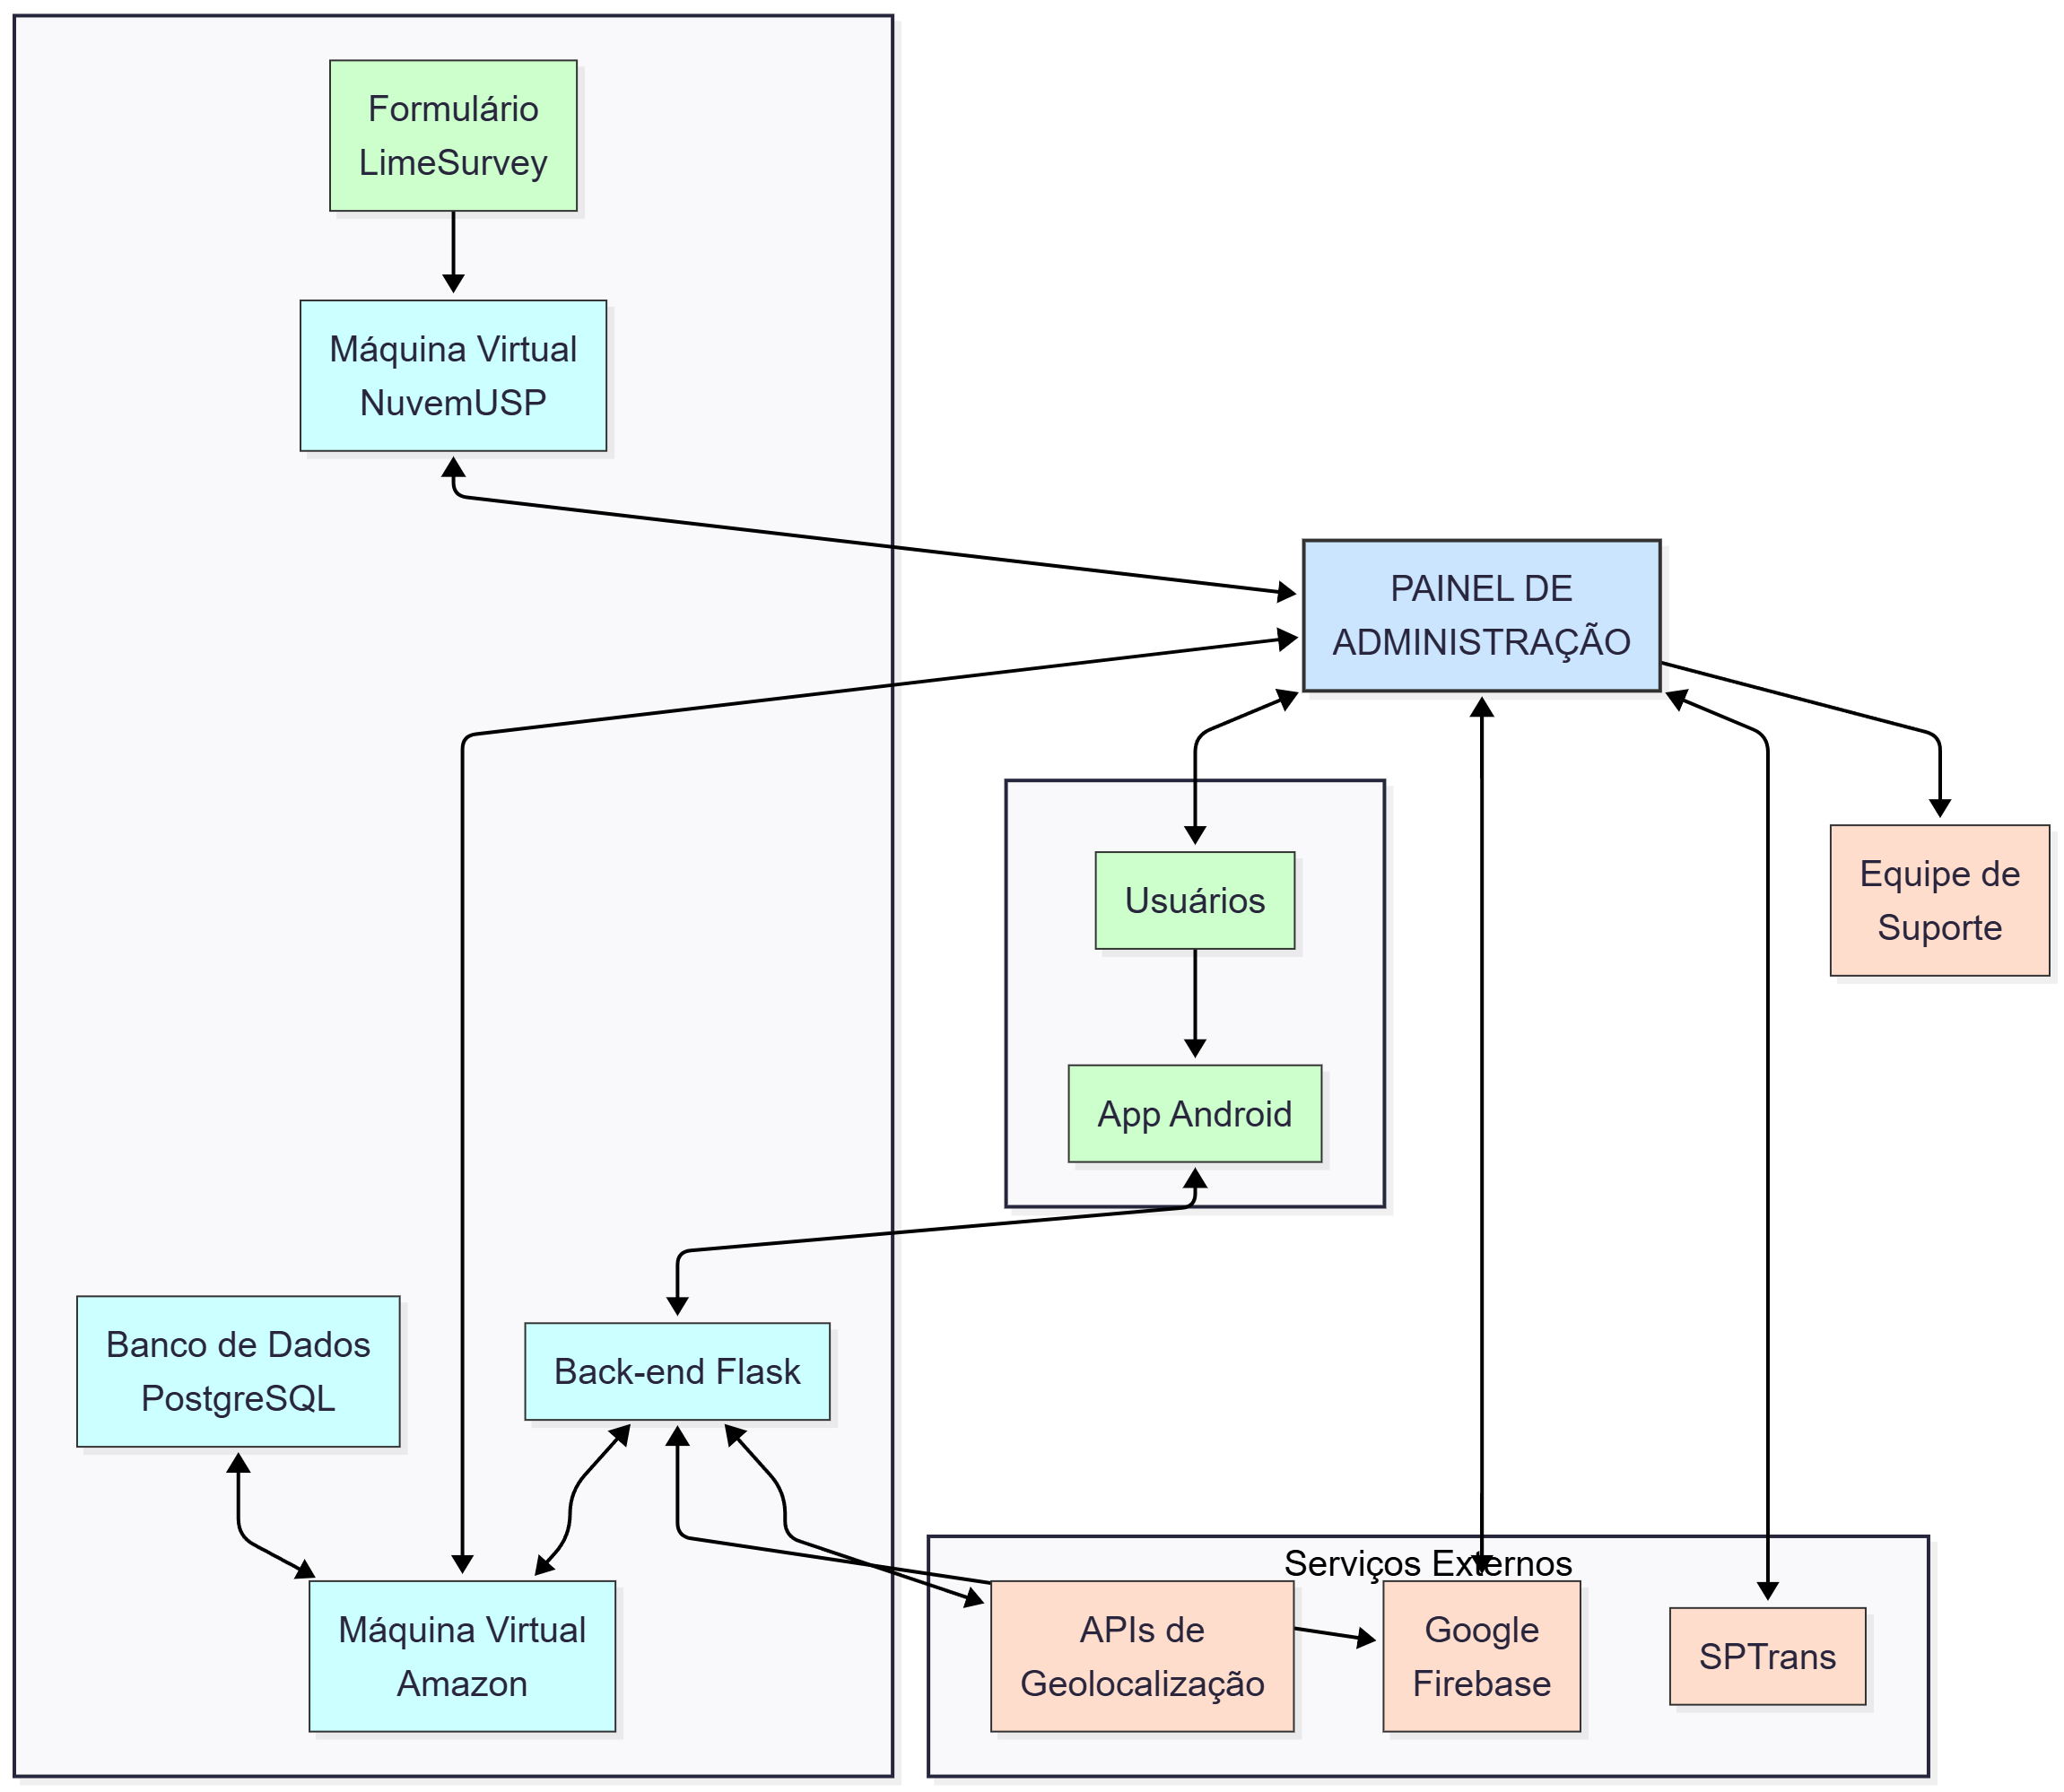
\includegraphics[width=0.95\textwidth]{diagrama_3.png}
  \caption{Diagrama simplificado dos componentes do sistema BikeSP.}
  \label{fig:arquitetura}
\end{figure}

\section{Processo de desenvolvimento}
\label{sec:processo-desenvolvimento}
O desenvolvimento envolveu múltiplos stakeholders e ciclos curtos de validação:
economistas (por exemplo, Thainá), suporte/atendimento (Sávio), coordenação e
orientação (Fábio e Paulo), além da equipe técnica. As demandas foram
priorizadas e acompanhadas via registro de \textit{issues}, criação de
\textit{pull requests} e revisão colaborativa, organizada no Gitlab, com homologação contínua durante
o pré-teste, o período de inscrições, a preparação de julho e a execução do
piloto.

\section{Abas do painel e uso no piloto}
\label{sec:abas-painel}

\subsection{Inserção de usuários}
%!TeX root=../tese.tex
%("dica" para o editor de texto: este arquivo é parte de um documento maior)

% Conteúdo da subseção sobre Inserção de Usuários
% Este arquivo é importado em 02-implementacao.tex

\textbf{Fluxo de inscrição e coleta de dados iniciais.} O processo de recrutamento de participantes para o piloto BikeSP iniciou-se com ampla divulgação midiática (entrevistas em jornais, redes sociais, site institucional), direcionando interessados para formulário online hospedado em instância LimeSurvey na NuvemUSP. O formulário coletava: dados pessoais (nome, CPF, email, data de nascimento, gênero), número do Bilhete Único (pré-requisito para participação, pois remuneração seria creditada neste cartão), senha para acesso ao aplicativo móvel, endereços textuais de até três localizações (tipicamente casa e trabalho/escola), telefone para contato, e concordância com Termo de Consentimento Livre e Esclarecido (TCLE --- documento obrigatório aprovado por Comitê de Ética para pesquisas envolvendo seres humanos). Durante o período de inscrições, o formulário recebeu aproximadamente 3.000 submissões, volume que requeria automação para transferência ao banco de dados PostgreSQL do sistema BikeSP.

\textbf{Script de inserção automatizada.} A funcionalidade de inserção em lote, acessível via botão ``Inserir Usuários!'' no painel administrativo, executa script que: (i) conecta à API do LimeSurvey e baixa todas respostas ainda não processadas; (ii) itera sobre cada resposta aplicando validações (CPF válido via algoritmo de verificação de dígitos, email em formato correto e único no sistema, Bilhete Único com 15 dígitos numéricos, senha com mínimo de caracteres configurável); (iii) criptografa a senha antes de armazenar (segurança crítica); (iv) geocodifica endereços textuais chamando APIs externas (TomTom, Google Maps, Nominatim OSM) para converter em coordenadas GPS; (v) armazena dados cadastrais da pessoa, vinculação do cartão Bilhete Único com status ativo, e coordenadas de casa e trabalho; (vi) atribui participante a coorte inicial (pode ser randomizado ou seguir configuração padrão); e (vii) registra logs detalhados de sucesso/falha para cada usuário processado.

Execução ocorre em thread separada (processamento assíncrono) para não bloquear interface administrativa durante operação (geocodificação via APIs externas é gargalo principal). Botão fica desabilitado durante processamento, prevenindo cliques duplos que iniciariam múltiplas execuções simultâneas. Mensagem inicial ``Usuários novos estão sendo inseridos!'' confirma início; mensagem final reporta quantidade inserida (``X usuários inseridos com sucesso'') ou erros encontrados.

\begin{figure}[H]
  \centering
  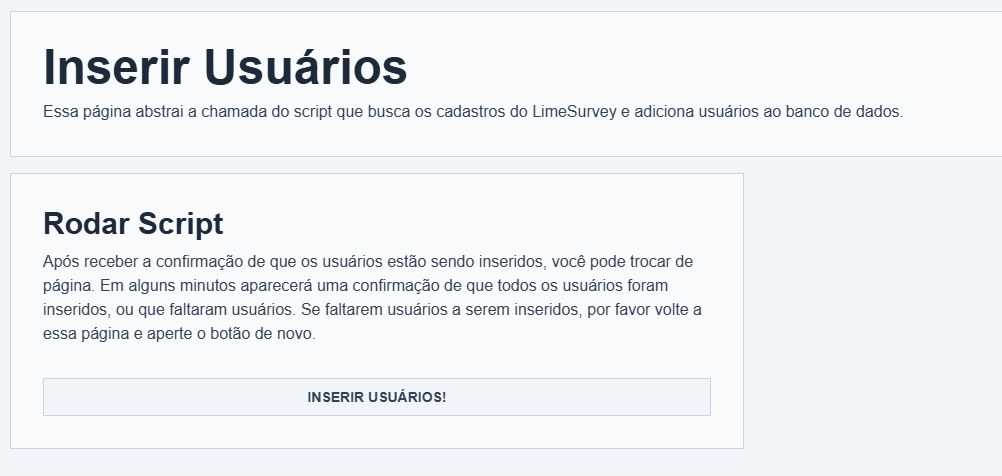
\includegraphics[width=0.95\textwidth]{figuras/inserir_usuarios.PNG}
  \caption{Interface de inserção de usuários no painel administrativo, com botão para executar o script de importação do LimeSurvey.}
  \label{fig:insercao_usuarios}
\end{figure}

\textbf{Tratamento de falhas e idempotência.} Sistema implementa verificação de CPF existente antes de tentar inserção, prevenindo duplicações mesmo se script executado múltiplas vezes sobre mesmas respostas do LimeSurvey (comportamento idempotente). Quando endereço falha em geocodificação (10-20\% dos casos conforme discussão na subseção de Localizações), localização é criada marcada como ``inválida'', permitindo participante existir no sistema mas impedindo uso daquela localização em viagens até correção manual via interface administrativa. Esta estratégia parcialmente otimista (criar usuário mesmo com dados incompletos) prioriza não bloquear participação --- melhor ter usuário com localização a corrigir que rejeitar inscrição completamente. Mensagens de aviso (``Y usuários faltaram a serem inseridos'', ``Z endereços não puderam ser geocodificados'') orientam reexecução do script (para tentar novamente usuários que falharam transientemente) e correção manual de localizações.

\textbf{Critérios de elegibilidade e seleção.} Embora formulário LimeSurvey coletasse ~3.000 inscrições, apenas 1.217 participantes foram efetivamente inseridos no sistema e incluídos no piloto. Critérios de elegibilidade aplicados durante seleção (manualmente por economistas antes de liberar CPFs para script de inserção) incluíam: residência em São Paulo (verificação via CEP), posse de Bilhete Único ativo, não ser cicloativista regular (auto-declaração --- para evitar viés de seleção, experimento buscava medir impacto em usuários representativos, não entusiastas pré-dispostos), e disponibilidade para participar durante seis meses. Preferência adicional para diversidade de perfis socioeconômicos e geográficos. Esta separação entre coleta ampla pelo LimeSurvey e inserção seletiva pelo script permitiu flexibilidade experimental mantendo integridade metodológica.

\textbf{Sincronização com atribuição de coortes.} Primeira execução do script, inserindo ~1.200 usuários simultaneamente, foi coordenada com atribuição inicial de coortes via funcionalidade de upload em lote (descrita na subseção de Coortes). Workflow combinado: economistas geravam CSV com (CPF, ID\_Coorte) aplicando randomização estratificada; administrador executava script de inserção LimeSurvey→PostgreSQL; aguardava confirmação de sucesso; imediatamente executava upload de atribuição de coortes; verificava balanceamento (~400 usuários por coorte); enviava notificações de boas-vindas via sistema de notificações. Este processo único e crítico ocorreu na véspera do início oficial do piloto, requirendo coordenação temporal precisa para permitir resolução de problemas antes que participantes recebessem instruções para ativar o aplicativo.

\textbf{Funcionalidade específica para o piloto.} Este processo de inserção em lote via script administrativo foi desenvolvido exclusivamente para o projeto piloto, onde era necessário selecionar manualmente 1.217 participantes dentre 3.000 inscritos aplicando critérios de elegibilidade (residência em São Paulo, não ser cicloativista, diversidade socioeconômica). O formulário LimeSurvey serviu como porta de entrada ampla para candidatos, enquanto o script de inserção permitia controle fino sobre quem seria efetivamente incluído no experimento controlado.

Para a implementação municipal em larga escala (~10.000-50.000 usuários), quando o programa BikeSP for liberado para todos os ciclistas de São Paulo, esta arquitetura de duas etapas (LimeSurvey → script → banco de dados) seria substituída por cadastro direto e automático via aplicativo móvel. Usuários interessados instalariam o aplicativo, preencheriam dados cadastrais diretamente na interface, e seriam automaticamente integrados ao sistema sem necessidade de aprovação ou processamento em lote por administradores. O formulário LimeSurvey e o script de inserção foram ferramentas necessárias apenas para o contexto experimental do piloto, não fazendo parte da arquitetura planejada para a política pública permanente.




\subsection{Usuários}
%!TeX root=../tese.tex
%("dica" para o editor de texto: este arquivo é parte de um documento maior)

% Conteúdo da subseção sobre Usuários
% Este arquivo é importado em 02-implementacao.tex

Durante o piloto BikeSP, com
aproximadamente 1.200 participantes selecionados dentre 3.000 inscritos, a equipe de
suporte enfrentava demandas diárias de atendimento. Questões como ``não consigo acessar o aplicativo'', ``minha viagem não foi
computada'', ``como altero meu endereço cadastrado'' requeriam identificação rápida
do participante no sistema para diagnóstico e resolução. A interface de gerenciamento
de usuários tornou-se, portanto, o
ponto de partida no sistema administrativo  para praticamente todas as operações de suporte,
auditoria e análise.

A tela de usuários apresenta
tabela com seis colunas principais: ID (identificador único), nome
completo, email, CPF, número do Bilhete Único, e indicador mostrando se o participante
completou o cadastro de senha (permitindo acesso ao aplicativo). O sistema consulta dados pessoais vinculados aos cartões Bilhete Único ativos, utilizando técnicas de otimização para obter contagem total sem sobrecarregar o banco de dados --- importante para responsividade em conjuntos de dados com milhares de registros. A coluna ``Tem Senha'' verifica se existe senha cadastrada para aquele usuário, indicador crucial para diagnosticar
problemas de acesso (usuário inscrito mas sem senha configurada não consegue entrar no aplicativo).

O sistema oferece busca unificada por nome
(parcial, \textit{case-insensitive}\@) ou ID exato.
Por exemplo, buscar ``silva'' retorna ``Silva João'', ``Silvana Costa'', ``Marcos da
Silva'', enquanto buscar ``123'' retorna apenas o participante com ID exatamente 123.
Esta abordagem dual (nome parcial vs. ID exato) equilibra flexibilidade para buscas
exploratórias (quando administrador conhece apenas nome aproximado) e precisão para
operações dirigidas (quando ID já foi identificado em interação anterior ou viagem
específica). Importante notar que a busca não cobre email, CPF ou Bilhete
Único diretamente; para localizar por estes atributos, utiliza-se ordenação combinada com inspeção visual. A Figura~\ref{fig:usuarios_listagem} apresenta a interface de listagem (dados fictícios para fins ilustrativos).


\begin{figure}[htb]
    \centering
    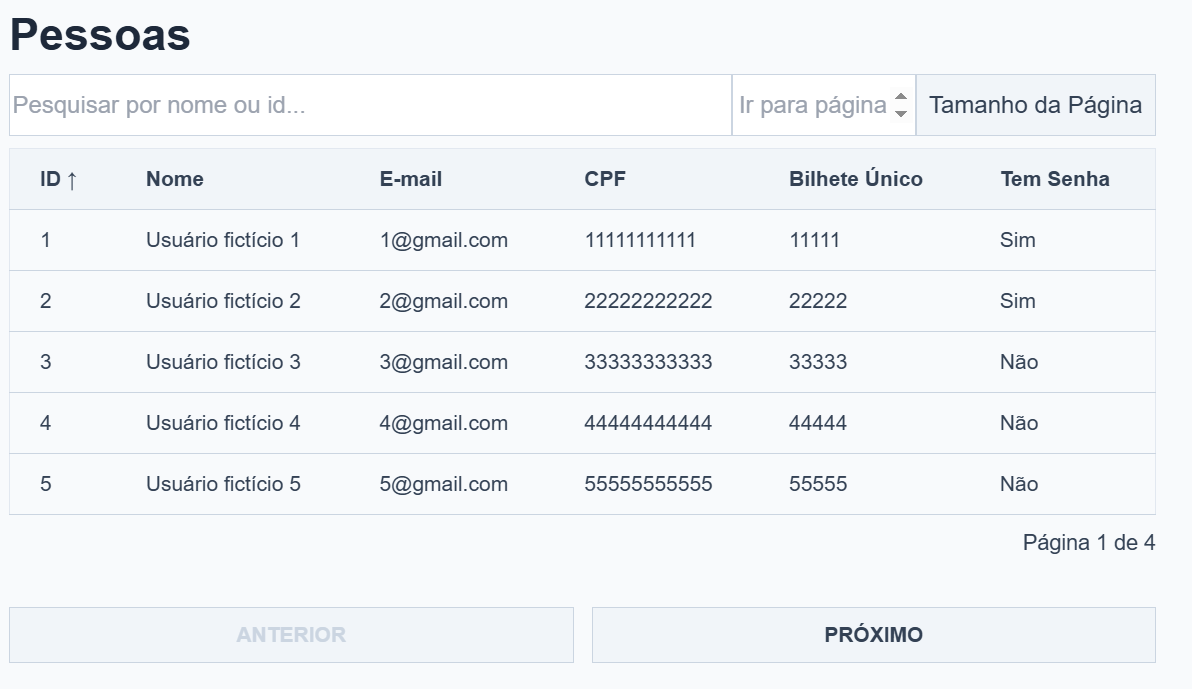
\includegraphics[width=0.95\textwidth]{figuras/pessoas.PNG}
    \caption{Interface de listagem de usuários com funcionalidades de busca, ordenação e paginação (dados fictícios).}
    \label{fig:usuarios_listagem}
  \end{figure}

Cada cabeçalho de coluna funciona como botão de
ordenação: primeiro clique ordena ascendentemente, segundo clique inverte para
descendente, com indicadores visuais (setas ↑↓) mostrando coluna ativa e direção.
Ordenação por nome facilita localização alfabética; por ID permite identificar
usuários cadastrados cronologicamente (IDs crescentes); por ``Tem Senha'' agrupa
participantes que completaram vs. não completaram ativação.

A interface oferece quatro densidades: 5, 10, 15
(padrão) ou 20 usuários por página, selecionáveis via dropdown. Navegação ocorre por
botões ``Anterior''/``Próximo'' (desabilitados nos extremos) ou campo de entrada
direta ``Ir para página X'', validando automaticamente se página solicitada existe.
Indicador ``Página X de Y'' fornece senso de escala do conjunto de dados. Esta
flexibilidade mostrou-se útil em diferentes contextos operacionais: densidade baixa
(5-10 itens) para inspeção cuidadosa com múltiplas abas abertas; densidade alta
(20 itens) para varredura rápida ou busca semi-manual quando termo de busca textual
não é aplicável.

A tela de usuários serve como ponto de
entrada para diversos fluxos operacionais críticos durante o piloto. \textit{Cenário
1: Suporte via email} --- participante reporta viagem não creditada; administrador
busca por nome, identifica ID, navega à tela de viagens filtrando por aquele ID,
localiza viagem em questão e diagnostica problema (ex: trajeto fora dos locais
cadastrados). \textit{Cenário 2: Problema de acesso ao app} --- participante não
consegue fazer login; administrador busca por nome, verifica coluna ``Tem Senha''; se
``Não'', orienta participante a completar cadastro via funcionalidade de redefinição
de senha. \textit{Cenário 3: Ajuste de localização} --- participante mudou de
endereço; administrador identifica ID, navega à tela de localizações, atualiza
coordenadas e endereço textual. \textit{Cenário 4: Contestação de viagem} ---
administrador recebe disputa; identifica usuário, obtém ID, acessa tela de
contestações para processar aprovação/rejeição. Em todos estes cenários, a rapidez
da busca e clareza da informação apresentada determinam eficiência do atendimento.

Durante o período de piloto, a
tela de usuários foi acessada diariamente pela equipe de suporte.
A métrica ``Tem Senha'' permitiu identificar participantes que não completaram ativação do aplicativo, 
orientando campanhas de engajamento. Recursos como ordenação e paginação reduziram significativamente a 
dependência de consultas manuais ao banco de dados, tornando as operações de suporte de primeiro nível mais ágeis
e acessíveis para toda a equipe.



\subsection{Coortes}
\label{sec:coortes}
%!TeX root=../tese.tex
%("dica" para o editor de texto: este arquivo é parte de um documento maior)

% Conteúdo da subseção sobre Coortes
% Este arquivo é importado em 02-implementacao.tex

O piloto BikeSP foi estruturado como experimento controlado randomizado (RCT --- \textit{Randomized Controlled Trial}) visando responder questão de implementação fundamental (IQ1): ``Como o número de viagens de bicicleta varia com diferentes valores de remuneração?'' Esta metodologia permite isolar efeito de incentivos financeiros de fatores confundidores, fornecendo evidências causais robustas para regulamentação da Lei Municipal 16.547/2016. Participantes foram alocados a três coortes (grupos experimentais) com diferentes níveis de remuneração por quilômetro pedalado: Coorte 0 (controle, sem remuneração), Coorte 1 (incentivo baixo, R\$~0,30/km, equivalente a 1/16 da tarifa de transporte público), e Coorte 2 (incentivo alto, R\$~0,60/km, equivalente a 1/8 da tarifa). A escolha destes valores baseou-se em estudo do Banco Mundial sobre elasticidade-preço de demanda por ciclismo em São Paulo, onde remunerações nesta faixa mostraram impacto significativo sem comprometer viabilidade orçamentária.

Característica distintiva do desenho foi rotação semanal de coortes: cada participante alternava entre as três condições a cada semana, experimentando todas coortes ao longo do piloto. Esta estratégia reduz viés de seleção (todos expostos a todas condições) e aumenta poder estatístico para detectar diferenças intra-indivíduos (cada participante serve como próprio controle). Adicionalmente, remuneração foi desativada em finais de semana para todas coortes, permitindo observar retenção de comportamento na ausência de incentivo financeiro --- descoberta notável foi que 9 das 10 viagens mais longas ocorreram justamente nestes períodos sem remuneração, evidência de internalização do hábito de pedalar.

A interface de coortes oferece funcionalidades para criação, listagem, e atribuição de participantes a grupos. Criação/atualização requer ID numérico único (1, 2, 3) e valor de remuneração por quilômetro; sistema automaticamente cria nova coorte se ID inexistente, ou atualiza valor se ID já cadastrado (útil para ajustes durante piloto sem recriar grupo). Listagem exibe ID, remuneração formatada como moeda (R\$~0,30), e quantidade de membros associados, com busca por ID específico e paginação (5 itens/página). Durante piloto com 1.217 participantes, distribuição manteve-se aproximadamente balanceada: ~400 participantes por coorte em qualquer semana dada, essencial para comparabilidade estatística.


 \begin{figure}[H]
   \centering
   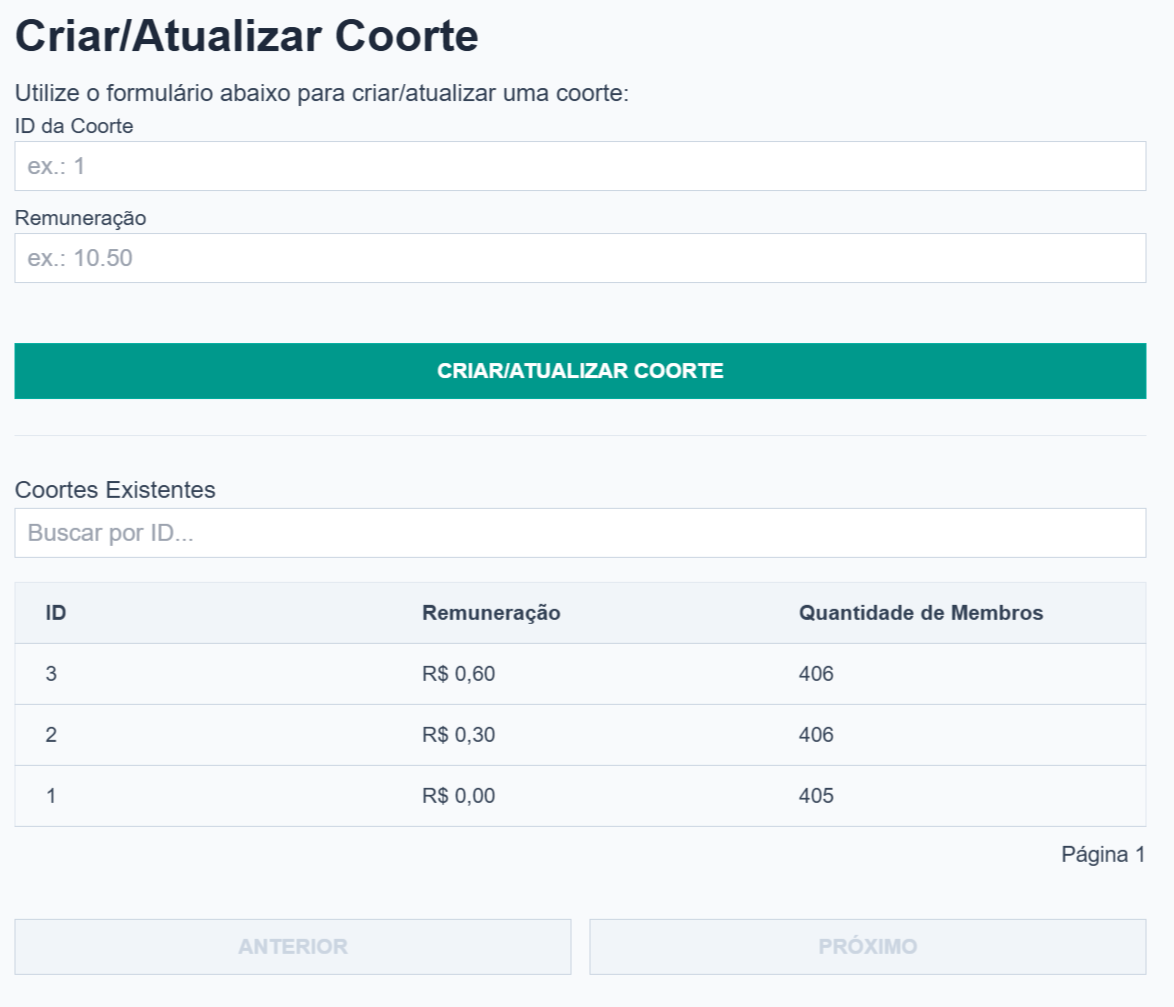
\includegraphics[width=0.95\textwidth]{figuras/coortes.PNG}
   \caption{Interface de gerenciamento de coortes e visualização de quantidade de participantes por grupo.}
   \label{fig:coortes_listagem}
 \end{figure}

 A tela dedicada lista todos usuários com respectivas coortes, exibindo ID, nome, email, total de viagens realizadas, e ID da coorte atual. Sistema de filtros combinados permite: busca por ID de pessoa, nome parcial (\textit{case-insensitive}), email, ID de coorte específica, e intervalo de viagens (mínimo/máximo). Filtros aplicam-se simultaneamente via lógica AND e persistem durante paginação. Esta funcionalidade atendeu múltiplos casos de uso: (i) verificar balanceamento de grupos (filtrar por ID de coorte, observar contagem); (ii) identificar participantes inativos (por exemplo, buscando com o filtro de usuários com no máximo 2 viagens); (iii) selecionar participantes altamente engajados para entrevistas qualitativas (por exemplo, buscando com o filtro de usuários com no mínimo 30 viagens); (iv) auditar atribuições após rotação semanal (exportar CSV, comparar com planilha esperada).

 \begin{figure}[H]
    \centering
    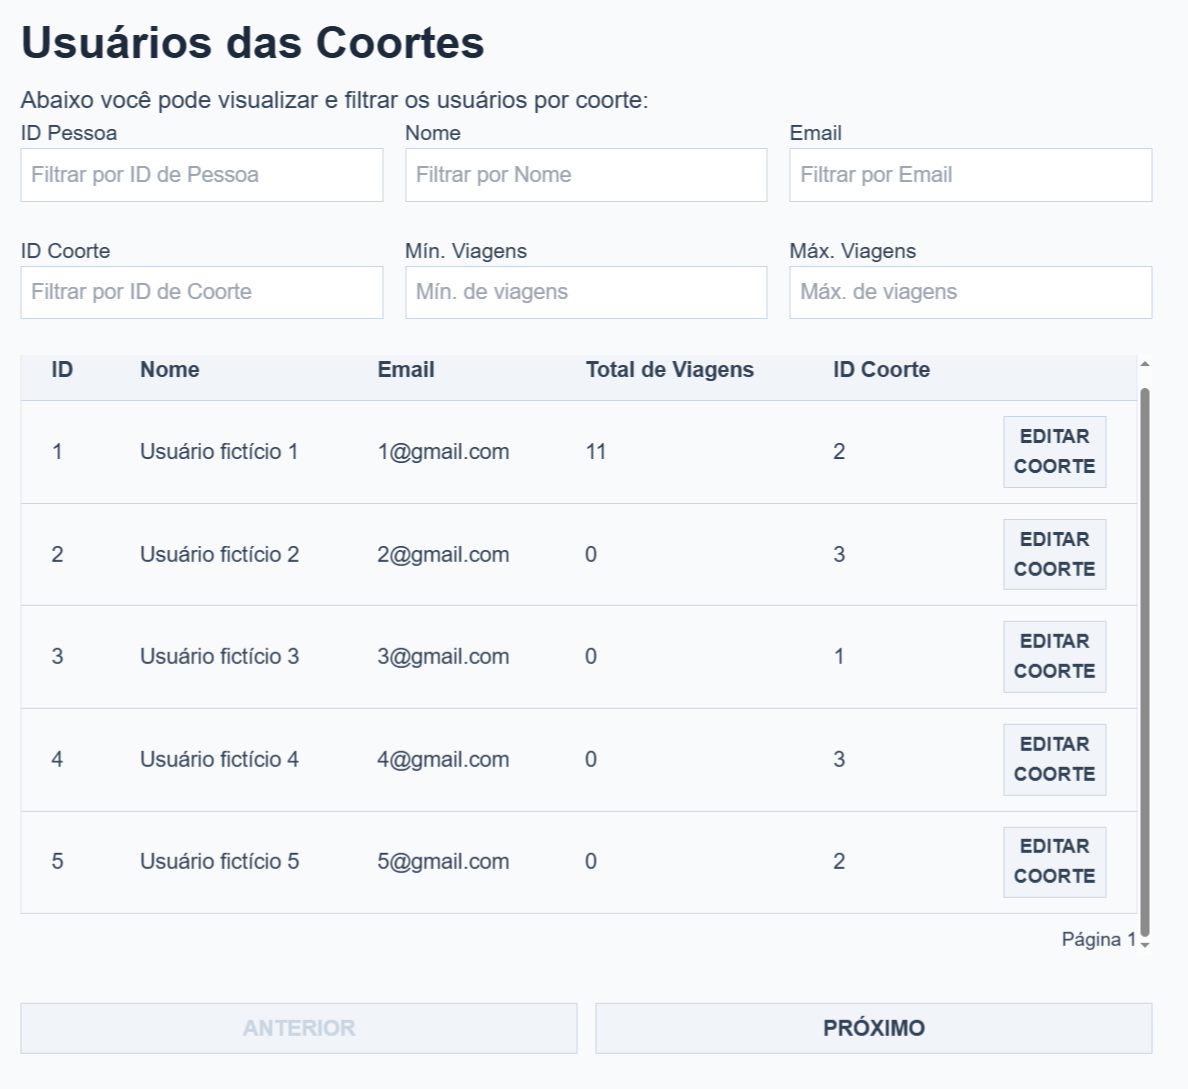
\includegraphics[width=0.95\textwidth]{figuras/usuario_coortes_zoom.PNG}
    \caption{Interface de filtragem de participantes por coorte.}
    \label{fig:coortes_listagem_usuarios}
  \end{figure}

Para correções pontuais, administrador pode editar coorte de usuário específico clicando ``Editar Coorte'' na linha da tabela, alterando ID para nova coorte ou deixando vazio para remover atribuição. Para operações em massa (rotação semanal), funcionalidade de upload via CSV permite atribuições em lote: arquivo com duas colunas (CPF;ID\_Coorte) separadas por ponto-e-vírgula, sem cabeçalho, codificação UTF-8. Sistema valida linha por linha antes de processar: CPF deve existir, coorte destino deve estar cadastrada, CPFs não podem duplicar. Erros específicos (``CPF 12345678901 não encontrado'', ``Coorte 99 não existe'') facilitam correção e reupload. Processamento atômico garante que ou todas atribuições são aplicadas ou nenhuma, prevenindo estados parciais que comprometeriam integridade experimental.

Durante piloto, rotação semanal típica seguia workflow: economistas geravam CSV com nova atribuição usando script (randomização estratificada por perfil socioeconômico e localização geográfica); administrador fazia upload via painel; sistema atualizava os registros; notificações push/email informavam participantes sobre nova remuneração vigente; exportação CSV pós-upload confirmava aplicação correta. Este processo de rotação semanal ao longo do projeto piloto evidenciou robustez e eficiência da funcionalidade.

\begin{figure}[H]
    \centering
    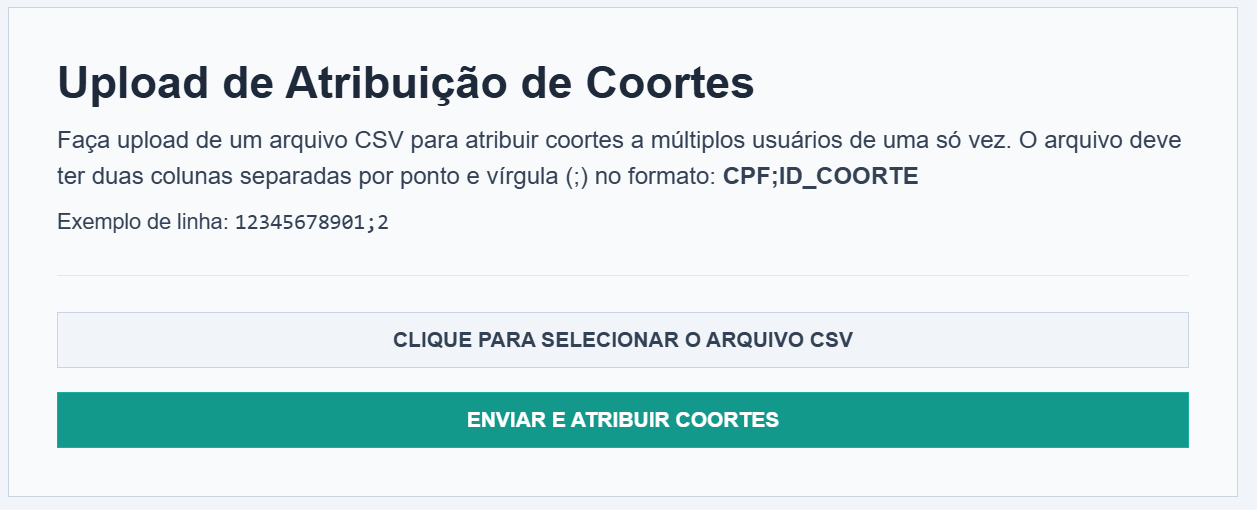
\includegraphics[width=0.95\textwidth]{figuras/upload_coortes.PNG}
    \caption{Interface de upload de atribuição de coortes em lote.}
    \label{fig:coortes_listagem_upload}
  \end{figure}

O botão de exportação gera CSV completo com ID, nome, CPF, email, ID da coorte, e valor de remuneração atual. O formato compatível com ferramentas estatísticas e facilita análises, o nome do arquivo gerado inclui a data da exportação, importante para criar um histórico versionado.

\begin{figure}[H]
    \centering
    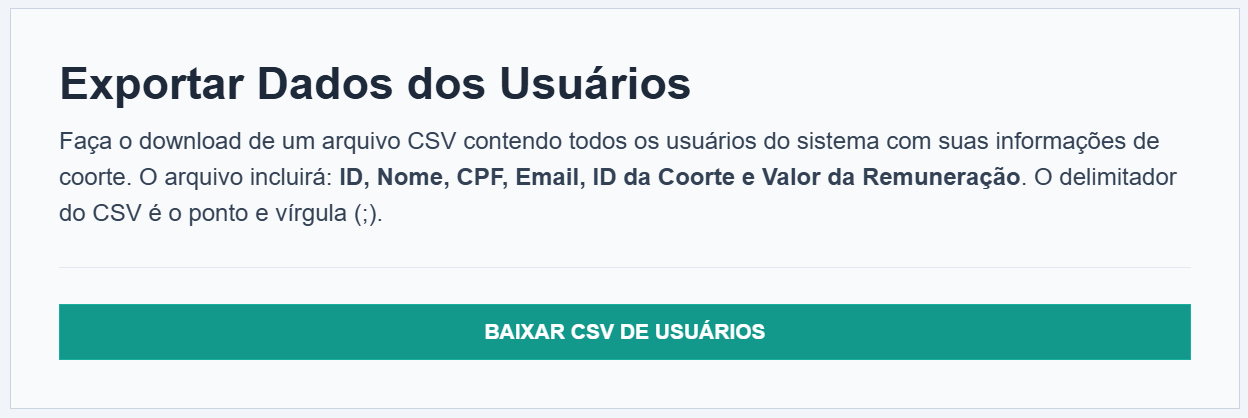
\includegraphics[width=0.95\textwidth]{figuras/exportar_coortes.PNG}
    \caption{Interface de exportação de coortes.}
    \label{fig:coortes_listagem_exportar}
  \end{figure}

O sistema implementa múltiplas salvaguardas: coortes não podem ser deletadas se possuem membros (previne perda acidental de atribuições); mudanças de remuneração em coorte ativa geram log detalhado (rastreabilidade de alterações durante experimento); tentativas de atribuir participante a coorte inexistente são rejeitadas (impossibilita referências órfãs); exportações registram timestamp e usuário que solicitou (auditoria de acesso a dados sensíveis).

A infraestrutura de gerenciamento de coortes no painel viabilizou análises sobre o impacto diferencial das remunerações. Os dados coletados durante o piloto permitirão investigar relações dose-resposta (comparando número de viagens entre diferentes valores de remuneração), validar a estratégia de rotação semanal, examinar retenção de participantes em cada coorte, e explorar heterogeneidade de efeitos por perfis socioeconômicos. Estas descobertas fundamentarão documento de recomendações para regulamentação da Lei Municipal 16.547/2016.





\subsection{Bônus}
\label{sec:bonus}
%!TeX root=../tese.tex
%("dica" para o editor de texto: este arquivo é parte de um documento maior)

% Conteúdo da subseção sobre Bônus
% Este arquivo é importado em 02-implementacao.tex

\textbf{Contexto e propósito dos bônus.} No contexto do piloto BikeSP, os bônus
representam uma ferramenta complementar de incentivo financeiro aos participantes,
independente das remunerações por quilômetro pedalado. Conforme planejado no desenho
do experimento, os bônus servem a múltiplos propósitos: (i) recompensar a conclusão
do curso gratuito ``Pedale com Segurança'' oferecido pelo Centro de Treinamento e
Educação de Trânsito (CETET) da CET; (ii) incentivar o preenchimento dos
questionários qualitativos aplicados em três momentos do piloto, garantindo maior
taxa de resposta e riqueza de dados; (iii) permitir ajustes administrativos e
correções pontuais de pagamento quando necessário; e (iv) viabilizar eventuais
campanhas promocionais temporárias para estimular a participação em momentos
estratégicos do experimento.

\textbf{Implementação técnica.} O painel administrativo oferece três
funcionalidades principais relacionadas a bônus: criação de novos tipos de bônus,
atribuição de bônus a usuários, e visualização e gerenciamento dos bônus
cadastrados. A arquitetura do sistema foi projetada para oferecer flexibilidade e controle sobre os incentivos.

\textbf{Criação de bônus.} Administradores podem cadastrar novos tipos de bônus
informando nome único (identificador), valor em reais, descrição textual, período
de validade (datas de início e fim, opcionais), e dois flags de controle: se o
bônus deve ser ativado automaticamente após criação, e se será visível aos
usuários no aplicativo móvel. A distinção entre bônus ativos/inativos e
visíveis/invisíveis oferece grande flexibilidade: bônus inativos não podem ser
concedidos (útil para pausar temporariamente um incentivo), enquanto bônus
invisíveis, mesmo quando concedidos e gerando remuneração, não aparecem na
listagem do aplicativo do usuário (útil para ajustes administrativos discretos ou
correções pontuais).

 \begin{figure}[H]
   \centering
   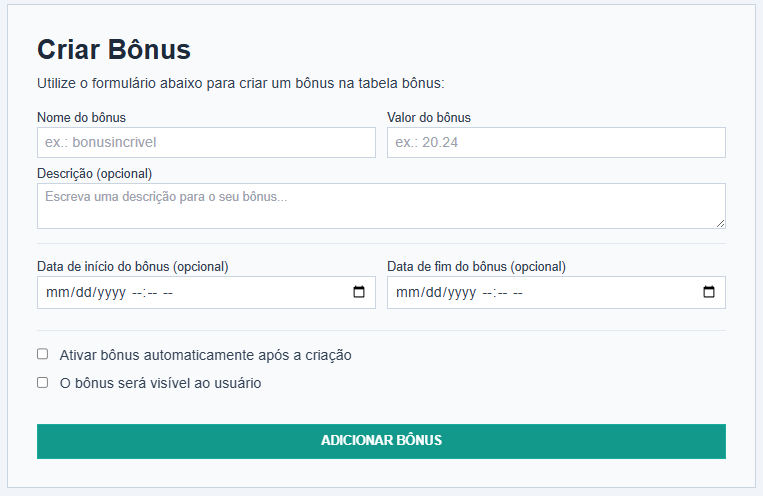
\includegraphics[width=0.95\textwidth]{figuras/criar_bonus.PNG}
   \caption{Formulário de criação de bônus no painel administrativo.}
   \label{fig:bonus_criar_form}
 \end{figure}

\textbf{Atribuição de bônus.} Para conceder um bônus a participantes, o
administrador informa os IDs dos usuários (separados por vírgula) e seleciona o
bônus desejado. O sistema valida diversas condições antes de processar a
concessão: o bônus deve estar ativo, não pode ter expirado (data de término não
ultrapassada), todos os usuários devem existir, e cada usuário pode receber cada
bônus apenas uma vez. Ao conceder um bônus com sucesso, o sistema não apenas registra a concessão, mas
também cria automaticamente uma remuneração correspondente ao valor do bônus e a
insere na fila de pagamentos (para posterior transferência aos cartões Bilhete
Único via Loja Virtual SPTrans). Caso algum usuário não atenda aos critérios, o
sistema reporta sucesso parcial, detalhando quantos usuários receberam o bônus e
quais apresentaram erros (por exemplo, ``5 sucesso(s), 2 erro(s): Usuário 101 já
possui este bônus; Usuário 203 não existe''). Esta funcionalidade de concessão em
lote reduz significativamente o tempo necessário para operações recorrentes, como
conceder o bônus do curso de segurança para todos os participantes que o
concluíram em determinada semana.

 \begin{figure}[H]
   \centering
   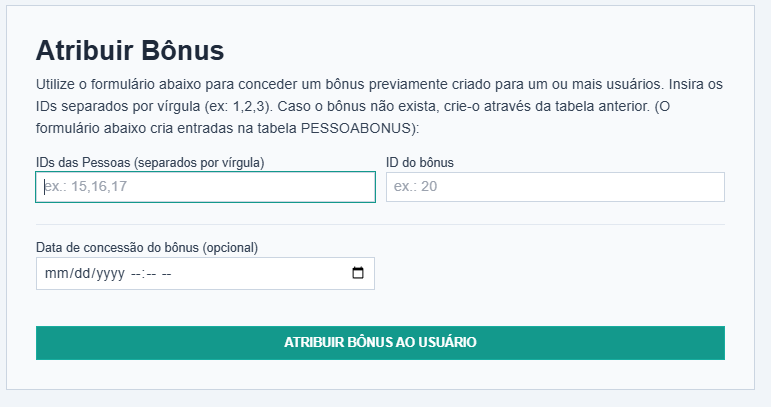
\includegraphics[width=0.95\textwidth]{figuras/atribuir_bonus.PNG}
   \caption{Formulário de atribuição de bônus aos participantes.}
   \label{fig:bonus_atribuir_form}
 \end{figure}

\textbf{Listagem e gerenciamento.} A tela de listagem exibe todos os bônus
cadastrados em formato tabular, apresentando ID, nome, valor, status de ativação,
visibilidade, descrição, período de validade e ações disponíveis. A interface
oferece busca por nome e paginação (5 itens por página). Cada linha da tabela
possui um botão para ativar ou desativar o bônus: bônus ativos exibem
botão vermelho ``Desativar'', enquanto bônus inativos exibem botão verde
``Ativar''. Importante notar que desativar um bônus não remove concessões já
realizadas nem afeta remunerações já geradas; apenas impede novas concessões
daquele tipo de bônus. Para facilitar a identificação dos IDs de usuários ao
atribuir bônus, a aba de bônus também oferece uma consulta integrada à tabela de
usuários, com busca por nome ou ID, ordenação por qualquer coluna e
paginação configurável da mesma forma que a tela de usuários.

\begin{figure}[H]
    \centering
    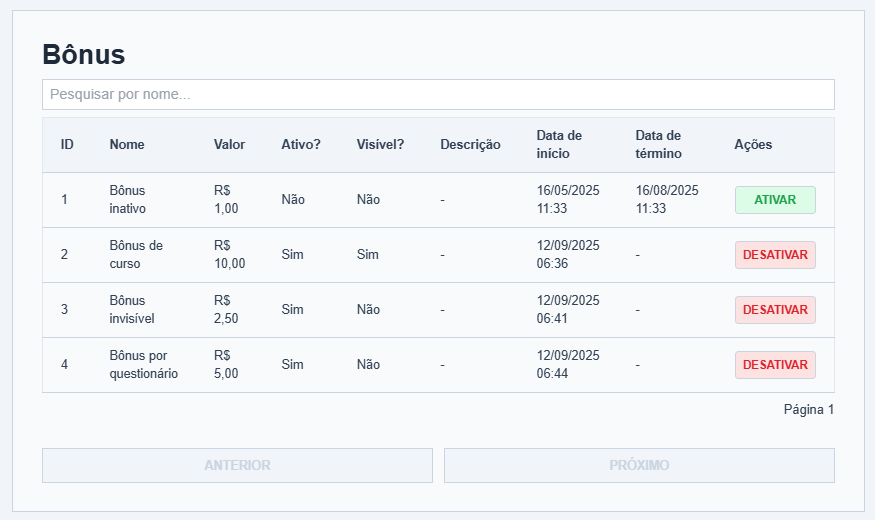
\includegraphics[width=0.95\textwidth]{figuras/bonus_listar.PNG}
    \caption{Listagem de bônus cadastrados com funcionalidades de busca, paginação e ativação/desativação.}
    \label{fig:bonus_listagem_form}
  \end{figure}
 

\textbf{Integração com o aplicativo móvel.} O aplicativo Android dos participantes
consome a API \texttt{POST /api/exibeBonus/} para listar os bônus concedidos ao
usuário autenticado. A API retorna apenas bônus marcados como visíveis, garantindo que ajustes administrativos invisíveis não
apareçam para os usuários finais. Esta separação entre visibilidade e concessão
oferece aos gestores do piloto a flexibilidade de realizar correções financeiras
sem necessariamente comunicá-las explicitamente aos participantes.

\textbf{Uso operacional no piloto.} Durante a execução do piloto, a
funcionalidade de bônus mostrou-se fundamental para diversos cenários operacionais:
concessão em lote do bônus do curso de segurança para centenas de participantes que
o concluíram simultaneamente; distribuição dos bônus dos questionários ao final de
cada período de coleta de dados qualitativos; correções pontuais quando erros de
geolocalização resultaram em viagens rejeitadas indevidamente (criando-se bônus
invisíveis de ajuste); A flexibilidade do sistema permitiu à
equipe operacional responder rapidamente a diferentes necessidades sem requerer
desenvolvimento de novas funcionalidades ou intervenções manuais no banco de dados.






\subsection{Remuneração}
\label{sec:remuneracao}
%!TeX root=../tese.tex
%("dica" para o editor de texto: este arquivo é parte de um documento maior)

% Conteúdo da subseção sobre Remuneração
% Este arquivo é importado em 02-implementacao.tex

A Lei Municipal 16.547/2016 estabeleceu
que o pagamento aos ciclistas do programa BikeSP seria realizado através de créditos
de transporte público, inseridos diretamente nos cartões Bilhete Único dos
participantes. Esta escolha reflete a intenção do governo municipal de integrar a
bicicleta ao sistema de transporte público, permitindo que os incentivos sejam
utilizados para deslocamentos multimodais (bicicleta + ônibus/metrô). O modelo de
remuneração por quilômetro pedalado, adotado também em iniciativas internacionais
como em Itajaí e na Holanda \citep{itajai2021, tennant2022}, visa recompensar a distância economizada ao
substituir outros modos de transporte, facilitando análises de impacto em poluição,
tráfego e saúde pública.

No desenho experimental do piloto, optou-se por valores de R\$~0,30 e R\$~0,60 por
quilômetro (equivalentes a 1/16 e 1/8 de uma passagem de transporte público,
respectivamente), com limite de duas viagens remuneradas por dia. Estes valores foram
baseados em estudo do Banco Mundial sobre disposição a pagar por ciclismo em São
Paulo \citep{worldbank2022}, que identificou que remunerações entre R\$~2,00 e R\$~3,00 por viagem
aumentavam em 38,4\% a probabilidade de escolher bicicleta sobre o modo atual,
efeito comparável à presença de ciclovias (43,4\%). A remuneração não foi
diferenciada por perfil de participante durante o piloto, pois um dos objetivos do
experimento era justamente compreender como o impacto da remuneração varia
segundo diferentes perfis demográficos e socioeconômicos.

O sistema de remuneração implementado no
painel administrativo gerencia três estados distintos do dinheiro: (i)
\texttt{aguardandoEnvio} --- valores de viagens aprovadas, bônus concedidos e
contestações deferidas que ainda não foram enviados à SPTrans; (ii)
\texttt{aguardandoResposta} --- valores já enviados à SPTrans através de arquivo
CSV, aguardando confirmação de creditação; e (iii) \texttt{concedido} --- valores
confirmados pela SPTrans como efetivamente creditados nos cartões Bilhete Único dos
participantes. Esta separação em estados permite rastreabilidade completa do fluxo
financeiro e reconciliação precisa entre solicitações, confirmações e valores
efetivamente pagos.

A funcionalidade de geração de CSV
para pagamento compila todos os valores em estado \texttt{aguardandoEnvio} de
participantes com Bilhete Único ativo. O arquivo gerado segue formato específico
exigido pela SPTrans: duas colunas delimitadas por ponto e vírgula (número do
Bilhete Único e valor), sem cabeçalho. O nome do arquivo inclui data e hora completa (exemplo:
\texttt{pagamentos05-10-2024-14-30-25.csv}) para garantir unicidade e
rastreabilidade. Ao gerar o CSV, o sistema automaticamente move os valores de
\texttt{aguardandoEnvio} para \texttt{aguardandoResposta}, evitando duplicação em
envios subsequentes. Esta operação é atômica e registrada em log para auditoria. A Figura~\ref{fig:remuneracao_gerar_csv_form_creditos} mostra a interface de geração.

\begin{figure}[H]
    \centering
    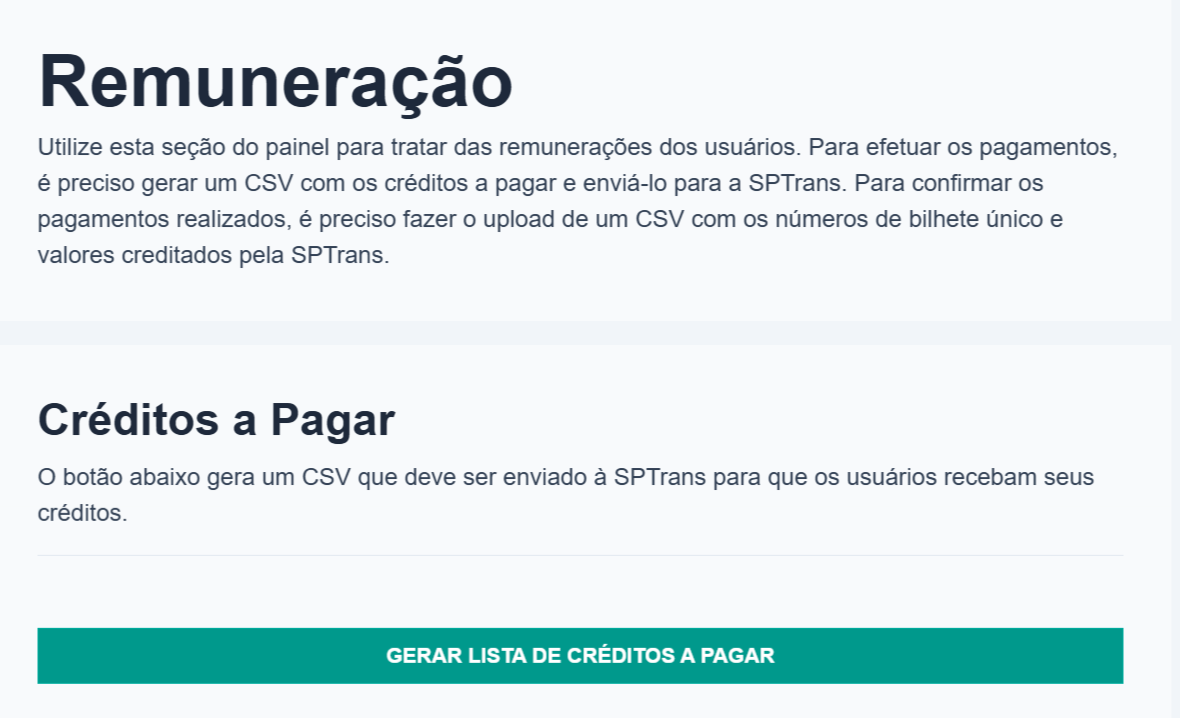
\includegraphics[width=0.95\textwidth]{figuras/remuneracao_creditos.png}
    \caption{Interface de geração de lista de créditos a pagar via SPTrans.}
    \label{fig:remuneracao_gerar_csv_form_creditos}
  \end{figure}

O arquivo CSV gerado é enviado
manualmente à SPTrans. A SPTrans credita os valores nos cartões Bilhete
Único dos participantes e retorna um arquivo CSV de comprovação contendo os bilhetes
efetivamente creditados e os valores pagos. Este processo manual, embora não
automatizado, mostrou-se adequado para a escala do piloto (cerca de 1.200
participantes) e garante supervisão humana sobre transações financeiras, reduzindo
riscos de erros sistêmicos em larga escala.



Ao receber o comprovante da SPTrans,
o administrador realiza upload do arquivo CSV no painel. O sistema executa validação
rigorosa linha por linha: verifica formato (exatas duas colunas), existência do
Bilhete Único no banco de dados, e validade numérica do valor. Qualquer erro
detectado aborta imediatamente o processamento completo, impedindo confirmações
parciais que poderiam gerar inconsistências. Apenas quando todas as linhas são
validadas com sucesso, o sistema processa a confirmação: move valores de
``aguardando resposta'' para ``concedido'', registra o histórico de pagamento como confirmado, e armazena a data e valor de cada operação. Mensagens específicas de erro (``Arquivo com
mais de duas colunas'', ``Formato incorreto de valor'', ``Bilhete não encontrado'')
facilitam correção rápida de problemas antes de reprocessar. A Figura~\ref{fig:remuneracao_gerar_csv_form_processados} ilustra a interface de upload.

\begin{figure}[H]
    \centering
    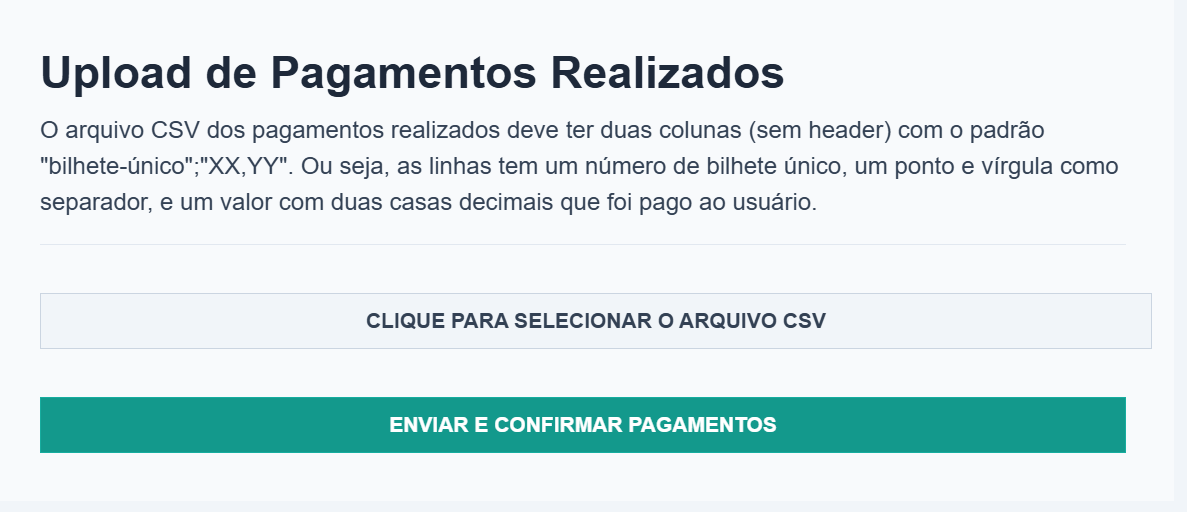
\includegraphics[width=0.95\textwidth]{figuras/remuneracao_processados.png}
    \caption{Interface de upload de comprovante de pagamentos realizados pela SPTrans.}
    \label{fig:remuneracao_gerar_csv_form_processados}
  \end{figure}
O sistema armazena, para cada Bilhete Único, os três estados de remuneração (concedido, aguardando envio, aguardando resposta) além da identificação do participante e status de ativação do cartão. Mantém também registro imutável de todos os envios de pagamento (identificados por número do bilhete e data), permitindo múltiplos pagamentos ao mesmo participante ao longo do tempo. Restrições do banco de dados garantem que valores sejam sempre não
negativos e que transições de estado sigam apenas fluxos
válidos. Toda operação financeira é registrada em log incluindo ID do administrador
responsável, garantindo trilha de auditoria completa e rastreabilidade para
conformidade com procedimentos do experimento.

O painel oferece visibilidade
sobre valores pendentes de envio, valores aguardando confirmação da SPTrans, e total pago aos participantes. 
Durante o piloto, estes indicadores foram fundamentais para
planejamento de fluxo de caixa e comunicação com participantes sobre prazos
esperados de creditação. 

O sistema contempla cenários
atípicos que ocorreram durante operação: (i) pagamentos parciais, quando SPTrans
credita valor inferior ao solicitado, mantendo diferença pendente de confirmação para reenvio posterior; (ii) bilhetes inválidos ou
bloqueados, que não aparecem no CSV de retorno da SPTrans e requerem investigação
manual com o participante; (iii) múltiplos pagamentos no mesmo dia, permitidos via
timestamp distinto na chave primária; e (iv) valores zerados no CSV, que são
ignorados sem gerar erro. A natureza atômica e idempotente do processamento de
confirmações permite reprocessar o mesmo CSV sem duplicações, útil em casos de
falhas de comunicação ou necessidade de revalidação.





\subsection{Contestações}
\label{sec:contestacoes}
%!TeX root=../tese.tex
%("dica" para o editor de texto: este arquivo é parte de um documento maior)

% Conteúdo da subseção sobre Contestações
% Este arquivo é importado em 02-implementacao.tex

O algoritmo de validação automática de viagens implementado no backend Flask rejeitava viagens que não atendiam critérios predefinidos: distância < 1km (consideradas muito curtas para deslocamento cotidiano), origem ou destino fora das localizações cadastradas (potencial fraude ou uso recreacional não remunerável), ou trajetória implausível (teletransportes indicando falha de GPS). Embora estes critérios reduzissem tentativas de fraude, geravam falsos positivos: viagem legítima rejeitada por erro temporário de GPS, localização ligeiramente deslocada devido a imprecisão de geocodificação, ou participante que iniciou pedalada próximo mas não exatamente na localização cadastrada. Sistema de contestações oferece canal para reverter rejeições injustas, balanceando a eficiência da automação com a supervisão humana.

No aplicativo móvel, participantes cujas viagens foram reprovadas visualizam botão ``Contestar'' na tela de detalhes da viagem. Ao clicar, preenchem campo de justificativa explicando por que consideram a viagem válida (ex: ``Saí de casa normalmente, mas GPS demorou para conectar'', ``Trabalho fica dentro de prédio comercial, endereço cadastrado é da entrada principal''). A contestação é enviada e cria registro com status pendente de análise, visível imediatamente na interface administrativa.

A tela administrativa de contestações exibe tabela paginada com ID da pessoa, ID da viagem, data, justificativa, e status (Pendente/Sim/Não). Busca textual cobre todos campos, útil para localizar contestações de participante específico (``busca: 123'') ou por palavra-chave na justificativa (``busca: GPS''). Ao clicar em linha, sistema destaca visualmente e carrega detalhes completos abaixo da tabela, incluindo nome do participante, justificativa integral, e mapa interativo renderizando trajeto GPS da viagem contestada. Visualização do trajeto revelou-se decisória: administrador constata se rota realmente conecta origem-destino, se passou por vias cicláveis, ou se apresenta anomalias (ex: linha reta implausível indicando falha de GPS). A visualização dos trajetos será melhor descrita na seção viagens. A Figura~\ref{fig:contestacoes_listagem} mostra a interface de listagem (dados fictícios para fins ilustrativos).

 \begin{figure}[H]
   \centering
   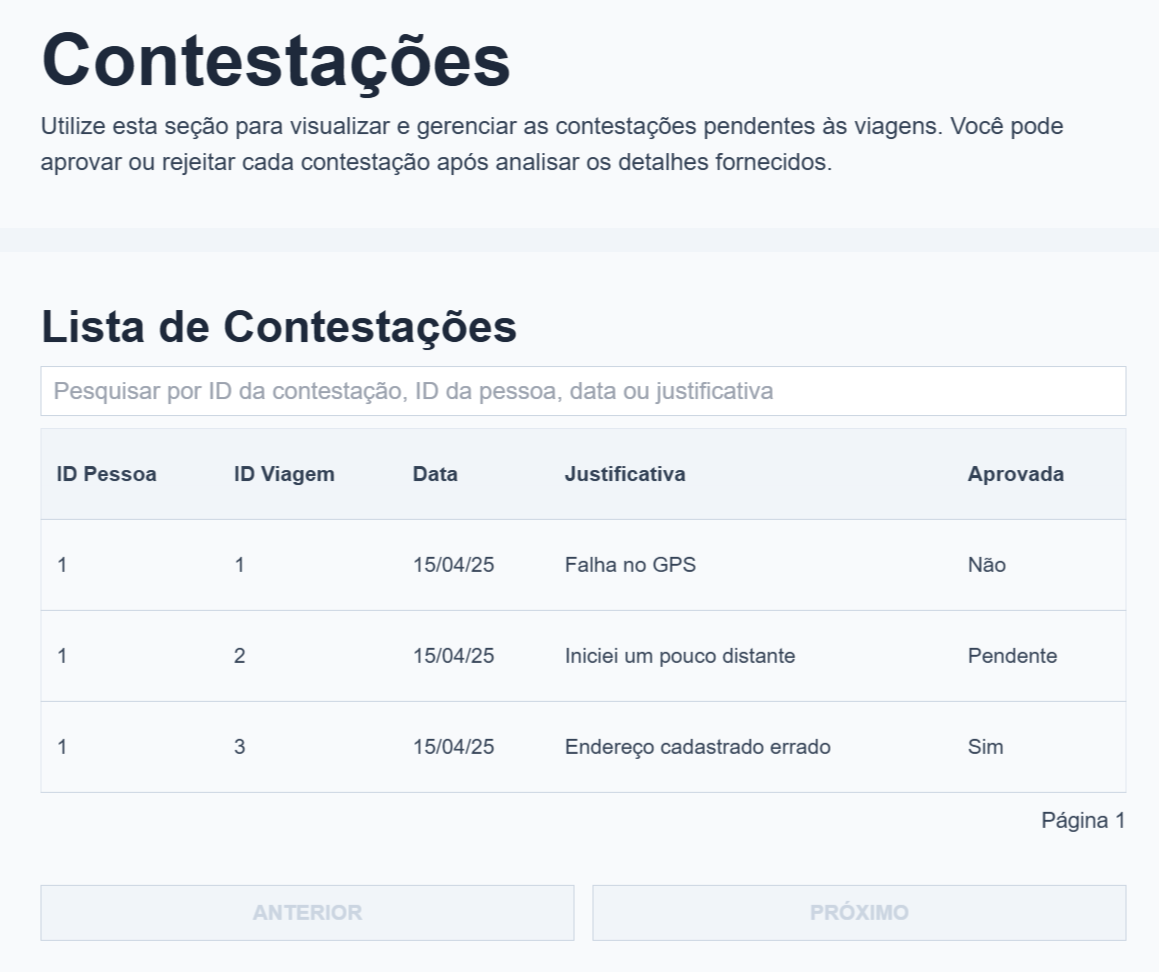
\includegraphics[width=0.95\textwidth]{figuras/contestacoes_listar.png}
   \caption{Interface de listagem de contestações com busca e paginação (dados fictícios).}
   \label{fig:contestacoes_listagem}
 \end{figure}



Após analisar mapa e justificativa, administrador pode aprovar contestação clicando botão com confirmação de duplo clique (prevenção contra aprovação acidental). Sistema executa validações adicionais: contestação não pode ter sido processada anteriormente, viagem deve ter origem e destino definidos e distintos, usuário deve estar em coorte ativa, e distância entre origem-destino $\geq$ 1km. Cálculo de remuneração segue fórmula oficial: \texttt{distancia\_km = min(8000, distancia\_metros) / 1000; remuneracao = distancia\_km * valor\_por\_km\_da\_coorte}. Distância é limitada em 8km (viagens mais longas recebem teto de 8km) para controlar orçamento. Ao aprovar, sistema: atualiza status da viagem para ``Aprovado'', salva valor de remuneração, adiciona crédito à fila de pagamentos, marca a contestação como aprovada, e opcionalmente salva resposta textual do administrador (feedback ao participante). Mensagem de sucesso confirma: ``Contestação da viagem 12345 aprovada com remuneração de R\$ 4,50''. A Figura~\ref{fig:contestacao_aprovar} ilustra a interface de aprovação/rejeição (dados fictícios para fins ilustrativos).

 
\begin{figure}[H]
    \centering
    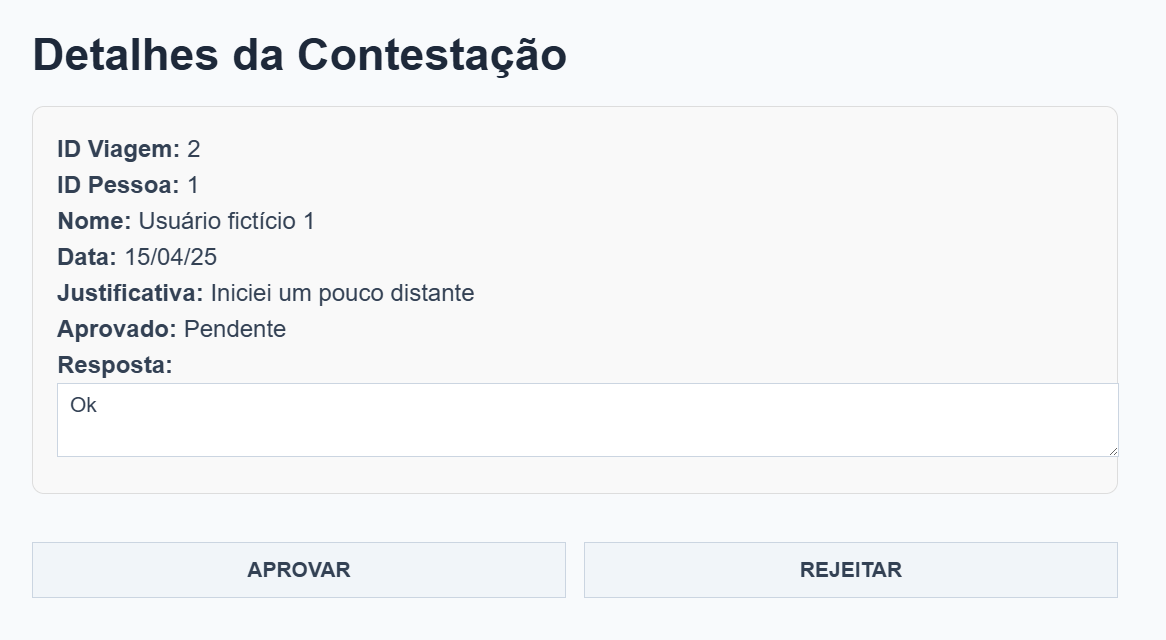
\includegraphics[width=0.95\textwidth]{figuras/contestacao_aprovar.PNG}
    \caption{Interface de aprovação/rejeição de contestação (dados fictícios).}
    \label{fig:contestacao_aprovar}
  \end{figure}

O administrador pode rejeitar contestação (também com confirmação dupla) quando: trajeto não conecta localizações cadastradas (participante tentou viagem recreacional), distância insuficiente mesmo com tolerância, ou justificativa indica má-fé (``não sabia que precisava ativar GPS''). Sistema atualiza contestação para reprovada, salva resposta opcional explicando motivo da rejeição (ex: ``Trajeto iniciou 2km distante da localização cadastrada. Por favor, inicie viagens próximo aos endereços registrados.''), e mantém viagem com status reprovado original. Campo de resposta é exibido no aplicativo móvel, permitindo participante compreender razão e ajustar comportamento futuro.

O sistema implementa múltiplas validações com mensagens específicas orientando correção: ``CONTESTAÇÃO INVÁLIDA'' (ID não encontrado), ``CONTESTAÇÃO JÁ GERENCIADA'' (processamento duplicado prevenido), ``VALOR FALTANDO PARA VIAGEM COM ORIGEM OU DESTINO DESCONHECIDO'' (dados incompletos na viagem), ``VALOR FALTANDO PARA VIAGEM COM ORIGEM == DESTINO'' (mesmo local), ``PESSOA SEM GRUPO PESQUISA'' (usuário não atribuído a coorte), ``DISTANCIA MENOR QUE 1KM'' (critério mínimo não atendido). Estas mensagens, além de prevenir estados inconsistentes no banco de dados, comunicam ao administrador qual condição falhou, permitindo diagnóstico e correção manual (ex: atribuir usuário a coorte antes de reaprovar contestação).



\subsection{Viagens}
\label{sec:viagens}
%!TeX root=../tese.tex
%("dica" para o editor de texto: este arquivo é parte de um documento maior)

% Conteúdo da subseção sobre Viagens
% Este arquivo é importado em 02-implementacao.tex

Durante os seis meses do piloto BikeSP, foram registradas mais de 29.000 viagens pelo aplicativo Android dos participantes, totalizando mais de 150.000 km pedalados. Este volume de dados demandou interface robusta para visualização, busca e análise pela equipe de suporte e pesquisadores. A tela de viagens tornou-se ferramenta essencial para diagnóstico de problemas reportados por usuários (``minha viagem não apareceu'', ``valor creditado está incorreto''), validação de contestações, e análises exploratórias para publicações científicas.

A tabela de viagens apresenta oito colunas principais: ID da viagem (identificador único), ID do usuário, data da viagem, deslocamento em metros, IDs de origem e destino (referenciando localizações cadastradas), status (aprovada/reprovada), e remuneração calculada em reais. O sistema consulta dados de viagens vinculando informações de pessoas e localizações de origem e destino, utilizando técnicas de paginação eficiente para responsividade. Ordenação padrão por ID decrescente exibe viagens mais recentes primeiro, padrão adequado para monitoramento operacional diário.

O campo de busca permite filtrar viagens por ID de usuário específico (busca exata). Esta funcionalidade atende cenário operacional frequente: participante relata problema com viagem; administrador identifica ID do usuário na tela de participantes; busca todas viagens daquele usuário; localiza a viagem em questão (geralmente reconhecível por data/horário ou trajeto).

 \begin{figure}[H]
   \centering
   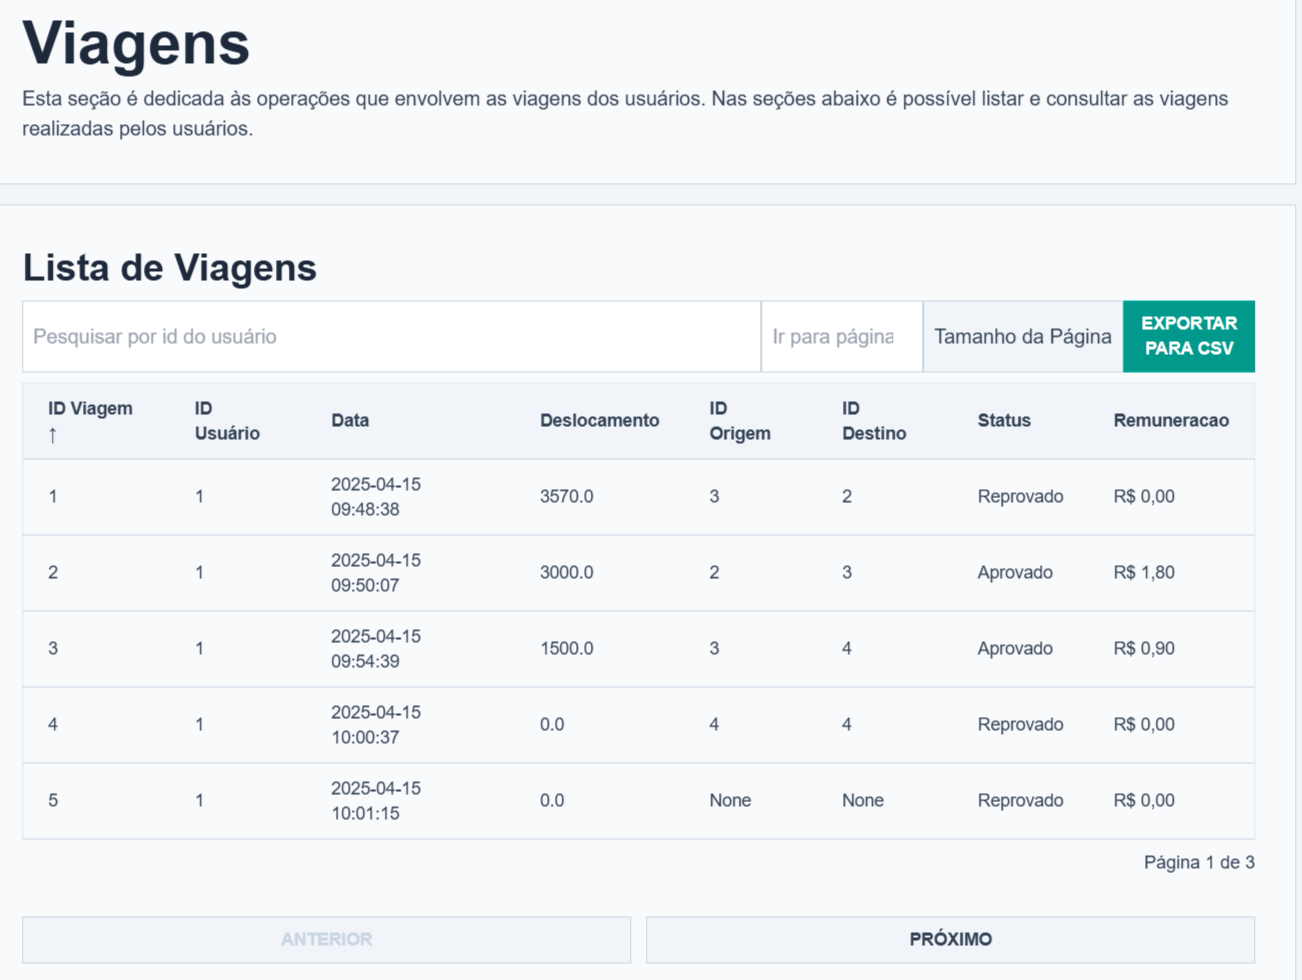
\includegraphics[width=0.95\textwidth]{figuras/viagens_listar.png}
   \caption{Interface de listagem de viagens com funcionalidades de busca, ordenação e paginação.}
   \label{fig:viagens_listar}
 \end{figure}

Ao clicar em qualquer linha da tabela, a interface renderiza mapa interativo (biblioteca Leaflet.js com tiles OpenStreetMap) exibindo trajeto completo da viagem abaixo da tabela. O mapa plota marcadores para cada ponto GPS coletado pelo aplicativo durante a viagem, conectados por linha azul na ordem temporal. Popups nos marcadores exibem timestamp de cada ponto. Zoom automático enquadra toda rota, e controles padrão (zoom, pan, scroll) permitem inspeção detalhada. Esta funcionalidade revelou-se crítica para validação de viagens contestadas: administradores visualizavam se trajeto realmente conectava origem e destino declarados, se passava por vias adequadas para ciclismo, e se não apresentava anomalias (ex: teletransportes indicando GPS incorreto).

\begin{figure}[H]
    \centering
    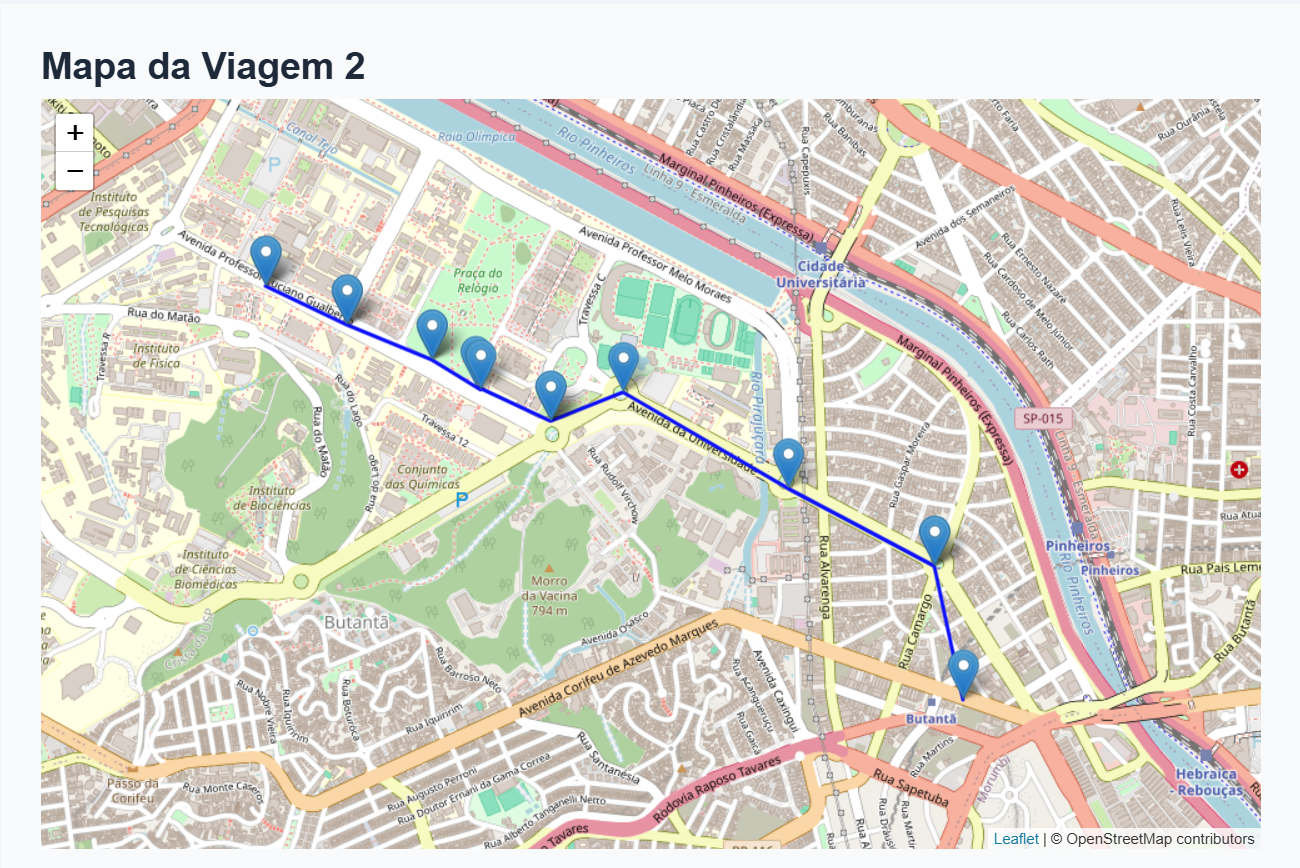
\includegraphics[width=0.95\textwidth]{figuras/mapa_contestacao.PNG}
    \caption{Visualização de trajeto de viagem fictícia com origem no IME e destino na estação Butantã no mapa interativo com marcadores de pontos GPS.}
    \label{fig:mapa_contestacao}
  \end{figure}

O botão de exportação gera arquivo CSV contendo todas as informações exibidas (respeitando filtros de busca ativos) para análise em ferramentas externas. O formato inclui cabeçalho descritivo e delimitador ponto-e-vírgula. Durante piloto, esta funcionalidade foi utilizada semanalmente por economistas do projeto para análises estatísticas: modelos de regressão investigando impacto das coortes no número de viagens, análises de série temporal identificando padrões de uso ao longo da semana, e visualizações geoespaciais em GIS identificando origens/destinos mais frequentes. A possibilidade de exportar dados filtrados (ex: apenas viagens de determinado usuário ou período) reduziu necessidade de consultas diretas ao banco de dados para análises.

A ordenação por diferentes colunas viabiliza análises rápidas: ordenar por deslocamento descendente identifica viagens mais longas (útil para identificar outliers ou comportamento atípico); ordenar por data permite inspeção cronológica (verificar se sistema registrou viagens durante manutenções); ordenar por status agrupa aprovadas vs. reprovadas (calcular taxa de aprovação manual); ordenar por remuneração identifica viagens de maior valor. Durante análise dos resultados do piloto, observou-se que 9 das 10 viagens mais longas (identificadas via ordenação por deslocamento) ocorreram em finais de semana sem remuneração, evidência importante de retenção intrínseca do hábito de pedalar para além do incentivo financeiro.

A configuração padrão de 10 viagens por página balanceia densidade de informação e tempo de carregamento. Com 29.000+ registros, carregar todas viagens simultaneamente seria inviável; paginação server-side (LIMIT/OFFSET no PostgreSQL) mantém responsividade independente do volume total. Indicador ``Página X de Y'' fornece senso de escala, reforçando necessidade de busca e ordenação para localizar informação relevante. Opções de 5, 15 ou 20 itens por página atendem diferentes casos de uso: densidade baixa para inspeção cuidadosa com múltiplos mapas abertos; densidade alta para varredura rápida de padrões.

\textit{Cenário 1: Diagnóstico de viagem não creditada} --- participante relata viagem realizada ontem não apareceu no extrato; administrador busca por ID do usuário, filtra viagens recentes (ordenação por data), identifica viagem com status ``reprovada''; visualiza mapa, constata que trajeto passou por localizações não cadastradas; orienta participante a atualizar endereços. \textit{Cenário 2: Validação de contestação} --- usuário contesta rejeição de viagem; administrador abre viagem contestada, visualiza mapa, confirma que trajeto conecta origem e destino cadastrados; aprova contestação, gerando remuneração retroativa.




\subsection{Notificações}
\label{sec:notificacoes}
%!TeX root=../Monografia - Mikhael Pinto.tex
%("dica" para o editor de texto: este arquivo é parte de um documento maior)

% Conteúdo da subseção sobre Notificações
% Este arquivo é importado em 02-implementacao.tex

%acho que teve comunicação nas coortes%
Com 1.217 participantes distribuídos geograficamente por São Paulo e engajados em experimento com rotação semanal de coortes, estabelecer canal eficaz de comunicação mostrou-se crítico. Eventos requerendo notificação incluíam: início de nova coorte (informar mudança de remuneração), disponibilidade de pagamento (créditos depositados no Bilhete Único), manutenções programadas no sistema, lembretes de preenchimento de questionários qualitativos, e esclarecimentos sobre regras do experimento após dúvidas recorrentes. Sistema de notificações implementado no painel oferece dois canais simultâneos: push notifications via Firebase Cloud Messaging (FCM) para aplicativo Android, e email via SMTP (Gmail) para endereços cadastrados.

A interface oferece três estratégias de direcionamento: (i) envio individual para IDs específicos separados por vírgula (ex: comunicação de suporte técnico, ``participantes 123, 456 e 789: problema reportado foi corrigido''); (ii) envio por coorte via IDs de grupos experimentais (ex: ``participantes da coorte 2: esta semana sua remuneração é R\$~0,60/km''); e (iii) broadcast para todos participantes cadastrados (ex: ``sistema em manutenção dia 15 das 02h-04h''). Esta granularidade atende necessidades distintas: comunicação individualizada reduz ruído para participantes não afetados; segmentação por coorte mantém integridade do desenho experimental (evitando confusão sobre qual valor de remuneração aplica-se a cada grupo); broadcast garante que informações críticas alcancem todos.

O formulário de criação requer título (usado como assunto de email e cabeçalho de push notification) e corpo da mensagem. Campo de corpo aceita HTML completo, permitindo formatação rica em emails: parágrafos (\texttt{<p>}), quebras de linha (\texttt{<br>}), negrito (\texttt{<strong>}), listas, e links. Suporte a HTML mostrou-se valioso para comunicações longas ou complexas, como FAQ respondendo dúvidas recorrentes ou instruções passo-a-passo para resolver problemas comuns. Push notifications, devido a limitações de espaço em dispositivos móveis, exibem apenas texto plano, adequado para mensagens concisas. Checkbox independentes para cada canal (push e/ou email) permitem escolher meio mais apropriado: push para alertas urgentes que requerem atenção imediata; email para informações detalhadas que usuário pode consultar posteriormente. A Figura~\ref{fig:notificacao_criar} mostra a interface de criação.

 \begin{figure}[htb]
   \centering
   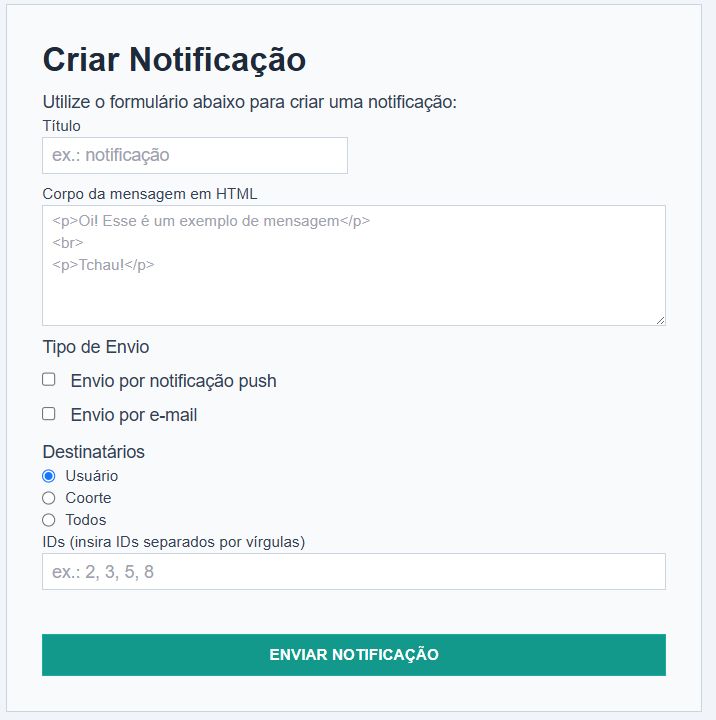
\includegraphics[width=0.95\textwidth]{figuras/notificacao_criar.PNG}
   \caption{Formulário de criação e envio de notificações para participantes.}
   \label{fig:notificacao_criar}
 \end{figure}

Para push notifications, o sistema consulta tabela de tokens FCM associados a cada participante (registrados durante primeira abertura do aplicativo), envia payload via API do Firebase, e notificação aparece na bandeja de notificações Android do participante. Falhas ocasionais ocorrem quando aplicativo é desinstalado ou token expira. Para emails, sistema busca endereços cadastrados, envia via protocolo SMTP autenticado em conta Gmail institucional, posicionando destinatários em BCC (cópia oculta para privacidade) e destinatário padrão configurável (tipicamente \texttt{bikesp-app@ime.usp.br}) no campo ``Para''. Esta arquitetura preserva privacidade (nenhum participante vê emails de outros) e profissionalismo (remetente institucional aumenta confiabilidade, reduzindo classificação como spam).

A funcionalidade de cópia oculta para email do administrador que enviou a notificação (mencionada em documentação como ``enviadas em cópia oculta para o email do administrador'') cria trilha de auditoria e permite verificação imediata de conteúdo e destinatários. Este registro mostrou-se útil para resolver disputas e manter histórico de comunicações para análise de engajamento.

O sistema valida que ao menos um canal (push ou email) está selecionado; que IDs de usuários/coortes são numéricos; e que campo de IDs é obrigatório apenas quando estratégia ``Usuário'' ou ``Coorte'' está selecionada (e escondida quando ``Todos'' marcado). Log de todas operações registra quem enviou, para quem, quando, e conteúdo da mensagem.

O sistema de notificações foi utilizado para diversos fins: broadcasts (anúncios gerais, disponibilidade de pagamentos), notificações por coorte (lembretes de remuneração ativa, instruções específicas), e mensagens individuais (suporte técnico, correções de problemas).




\subsection{Localizações}
\label{sec:localizacoes}
%!TeX root=../Monografia - Mikhael Pinto.tex
%("dica" para o editor de texto: este arquivo é parte de um documento maior)

% Conteúdo da subseção sobre Localizações
% Este arquivo é importado em 02-implementacao.tex

O desenho do experimento BikeSP especificou que apenas viagens entre localizações pré-cadastradas seriam remuneradas, visando incentivar deslocamentos cotidianos (casa-trabalho, casa-escola) em detrimento de viagens recreacionais irregulares. Durante inscrição via formulário LimeSurvey, participantes forneciam endereços textuais de até três localizações principais (tipicamente residência, trabalho/estudo, e uma terceira opcional). O sistema realizava geocodificação automática destes endereços  --- conversão de texto (``Av. Paulista, 1000, Bela Vista, CEP 01310-100'') para coordenadas GPS (latitude/longitude) utilizando APIs externas de geolocalização.

Para prevenir fraudes (participante alterando localizações para simular viagens longas fictícias), implementou-se regra de uma única alteração por localização após cadastro inicial. Participante que cadastrasse endereço incorreto ou mudasse de residência/trabalho poderia corrigi-lo uma vez via aplicativo; segunda tentativa de alteração seria bloqueada. Esta restrição, embora necessária para integridade experimental, gerou demandas de suporte quando usuários cometiam erros tipográficos ou mudavam endereço legitimamente após já terem usado sua cota de alteração.

A interface administrativa de localizações permite buscar por ID de participante e visualizar todas localizações cadastradas (ID, endereço completo, coordenadas, tipo). Funcionalidade crítica é reset da permissão de alteração: administrador, após validar legitimidade da solicitação via email ou telefone, pode remover o registro que controla alterações de localização, concedendo ao participante nova oportunidade de modificar endereço no aplicativo. Mensagens de feedback (``O usuário agora pode trocar uma localização'' vs. ``Nenhuma alteração de localização foi encontrada'') informam sucesso ou ausência de restrição ativa. Este procedimento foi utilizado durante o piloto, geralmente após mudanças residenciais ou correções de erros de digitação durante inscrição inicial.

Durante o script de inserção em lote de participantes do LimeSurvey para PostgreSQL, alguns endereços falhavam em geocodificação automática. Causas possíveis incluíam: formatação inconsistente (``Rua X, 100'' vs. ``Rua X|100|...''), abreviações não reconhecidas, bairros incorretos, CEPs inválidos, endereços recém-criados ausentes em bases cartográficas, e timeouts de APIs. Localizações que falhavam geocodificação eram marcadas como ``inválidas'' e ficavam inacessíveis no aplicativo móvel ---  participante visualizava localização na lista mas não podia utilizá-la como origem/destino de viagens, bloqueando efetivamente sua participação.

Este problema revelou-se crítico: correção manual urgente foi necessária durante o piloto. A funcionalidade de correção de geolocalização tornou-se operação essencial.

A tela de localizações inválidas lista endereços que falharam, exibindo ID, ID do participante, endereço textual, tipo e apelido da localização. Funcionalidades de busca, ordenação e paginação seguem padrão estabelecido em outras telas. Para corrigir, administrador edita endereço diretamente seguindo dois formatos possíveis: (i) endereço estruturado separado por pipe (ex: \texttt{Av. Paulista|1000|sala 5|Bela Vista|01310-100|São Paulo|SP}), submetido novamente às APIs de geocodificação; ou (ii) coordenadas GPS diretas (ex: \texttt{-23.5997136,-46.4677964}), sem precisar passar pela geocodificação quando endereço é intratável por APIs mas localização é conhecida via Google Maps. Validação bem-sucedida remove localização da lista de inválidas, tornando-a imediatamente disponível no aplicativo do participante.

Workflow operacional típico incluía: cópia do endereço para Google Maps, verificação de formatação e bairro correto, ajuste se necessário, validação no sistema. Problemas recorrentes e soluções documentadas: CEPs com dígitos transpostos (buscar CEP correto online); bairros coloquiais vs. oficiais (Pinheiros vs. Alto de Pinheiros); abreviações (``Av.'' expandir para ``Avenida''); endereços inexistentes (usar coordenadas GPS obtidas manualmente). A disponibilidade de múltiplas APIs de geolocalização aumentava taxa de sucesso, mas timeouts ocasionais justificavam opção de inserção direta de coordenadas.

A correção de localizações inválidas foi realizada pela equipe de suporte. Diferentes abordagens foram utilizadas: reformatação com nova geocodificação automática, inserção manual de coordenadas diretas obtidas via Google Maps, ou contato com participante para clarificação de endereço.

Para iterações futuras do programa, recomendações incluem: validação de formato durante preenchimento do formulário LimeSurvey, geocodificação imediata após submissão do formulário com feedback visual ao candidato, e assistente de endereçamento integrado (autocompletar baseado em API de CEPs). A natureza manual e laboriosa da correção em lote demonstrou ser gargalo operacional não escalável: expansão para 10.000 participantes (meta de implementação municipal completa) seria inviável sem automação adicional nesta etapa.




Após a descrição detalhada da implementação do painel administrativo e suas funcionalidades, o próximo capítulo apresenta os resultados alcançados durante a execução do piloto, incluindo dados quantitativos de uso e uma avaliação do impacto do sistema nas operações.


%!TeX root=../tese.tex
%("dica" para o editor de texto: este arquivo é parte de um documento maior)

\chapter{Resultados e avaliação}
\label{cap:resultados}

Este capítulo apresenta os resultados alcançados durante a execução do piloto BikeSP. A Seção~\ref{sec:resultados-atingidos} descreve os números e conquistas do experimento, incluindo volume de viagens, participação e descobertas relevantes. A Seção~\ref{sec:analise} apresenta uma análise de como o painel administrativo apoiou as perguntas de pesquisa e a execução do piloto.

\section{Resultados atingidos}
\label{sec:resultados-atingidos}
O piloto alcançou resultados expressivos em termos de coleta de dados e
engajamento dos participantes. Durante o pré-teste e o piloto, houve
\textbf{coleta intensiva de dados} via aplicativo e painel ao longo de cerca de
\textbf{dois meses} (julho e agosto). Os números do experimento foram:
\begin{itemize}
  \item \textbf{3~mil inscrições} recebidas no processo seletivo;
  \item \textbf{1217 participantes} selecionados para o experimento;
  \item \textbf{Mais de 29~mil viagens} registradas pelo aplicativo durante o
        experimento;
  \item \textbf{Mais de 150~mil quilômetros} pedalados no total.
\end{itemize}

Um resultado particularmente relevante foi a \textbf{retenção no uso do
aplicativo mesmo sem remuneração}. Entre as 10 viagens mais longas registradas,
9 foram realizadas fora dos períodos de remuneração (finais de semana),
indicando engajamento genuíno dos participantes com o sistema e com a prática do
ciclismo urbano, independentemente do incentivo financeiro imediato.

O projeto foi considerado um sucesso operacional. Em julho, o painel foi usado
para acompanhar o uso e prestar atendimento a usuários com dificuldades; em
agosto, executou-se o piloto principal em quatro semanas. A partir do segundo
teste com cerca de 40 participantes, foram mapeadas novas funcionalidades
críticas. Entre elas, destaca-se a \textbf{página do painel dedicada a corrigir
erros de geolocalização}, cuja operação reduziu consideravelmente as reclamações
dos usuários, permitindo que a equipe de suporte resolvesse problemas técnicos
de forma ágil e eficiente.

Entre os ganhos observados com o uso do painel:
\begin{itemize}
  \item \textbf{Eficiência}: atribuição de bônus em lote e ações em linha
        reduziram etapas repetitivas e tempo operacional.
  \item \textbf{Qualidade da informação}: padronização de datas/estados e
        visões dedicadas (Pessoas, Coortes) elevaram a confiabilidade das
        consultas e relatórios.
  \item \textbf{Governança}: listas de pagamento com trilhas de decisão e
        histórico de contestações facilitaram auditoria e reconciliação.
  \item \textbf{Suporte ao usuário}: ferramentas de correção de dados
        (especialmente geolocalização) reduziram reclamações e melhoraram a
        experiência dos participantes.
\end{itemize}


\section{Análise}
\label{sec:analise}
Como o painel apoia as perguntas de pesquisa e a execução do piloto \citep{interscity:pilotoBikeSP}.

O próximo capítulo conclui este trabalho, destacando as principais contribuições e discutindo possibilidades de trabalhos futuros e expansão do sistema.



%!TeX root=../Monografia - Mikhael Pinto.tex
%("dica" para o editor de texto: este arquivo é parte de um documento maior)

\chapter{Conclusão}
\label{cap:conclusao}

Este trabalho apresentou o contexto do programa Bike~SP e a implementação de um
painel administrativo para apoiar o piloto. As principais contribuições foram a
estruturação de módulos voltados à operação e análise de dados, alinhados ao
desenho experimental documentado \citep{faria2023:bikespCaseStudy}.

O sistema desenvolvido permitiu a coleta bem-sucedida de dados de mais de 30~mil
viagens e o gerenciamento operacional de 1217 participantes ao longo de quatro
semanas de experimento. Os dados coletados através do software desenvolvido
serão essenciais para a elaboração de um \textbf{documento de recomendações para
a regulamentação da Lei Municipal 16.547/2016} em São Paulo, fornecendo
evidências empíricas sobre a efetividade de diferentes níveis de incentivo
financeiro na promoção do ciclismo urbano.

Os resultados positivos do piloto abrem possibilidades para trabalhos futuros,
incluindo: (i) adaptação do sistema para suportar um número maior de
participantes na implantação em larga escala do programa em São Paulo; (ii)
replicabilidade do sistema em outras cidades --- o sistema está sendo
considerado para adoção pela Prefeitura de Fortaleza, o que demandará adaptações
e generalizações do código; (iii) estudos aprofundados sobre os padrões de
mobilidade identificados, perfis de usuários e efetividade comparativa dos
diferentes níveis de incentivo; e (iv) refinamento contínuo das funcionalidades
do painel com base no feedback da equipe operacional e dos pesquisadores.

A experiência adquirida no desenvolvimento e operação deste painel demonstra o
papel fundamental de ferramentas administrativas bem projetadas na viabilização
de experimentos científicos de políticas públicas de mobilidade urbana.





%%%%%%%%%%%%%%%%%%%%%%%%%%%% APÊNDICES E ANEXOS %%%%%%%%%%%%%%%%%%%%%%%%%%%%%%%%

% Um apêndice é algum conteúdo adicional de sua autoria que faz parte e
% colabora com a ideia geral do texto mas que, por alguma razão, não precisa
% fazer parte da sequência do discurso; por exemplo, a demonstração de um
% teorema intermediário, as perguntas usadas em uma pesquisa qualitativa etc.
%
% Um anexo é um documento que não faz parte da tese (em geral, nem é de sua
% autoria) mas é relevante para o conteúdo; por exemplo, a especificação do
% padrão técnico ou a legislação que o trabalho discute, um artigo de jornal
% apresentando a percepção do público sobre o tema da tese etc.
%
% Os comandos appendix e annex reiniciam a numeração de capítulos e passam
% a numerá-los com letras. "annex" não faz parte de nenhuma classe padrão,
% foi criado para este modelo. Se o trabalho não tiver apêndices ou anexos,
% remova estas linhas.
%
% Diferentemente de \mainmatter, \backmatter etc., \appendix e \annex não
% forçam o início de uma nova página. Em geral isso não é importante, pois
% o comando seguinte costuma ser "\chapter", mas pode causar problemas com
% a formatação dos cabeçalhos. Assim, vamos forçar uma nova página antes
% de cada um deles.

%%%% Apêndices %%%%

\cleardoublepage

\pagestyle{appendix}

\appendix

% \addappheadtotoc acrescenta a palavra "Apêndice" ao sumário; se
% só há apêndices, sem anexos, provavelmente não é necessário.
% \addappheadtotoc  % Comentado temporariamente para evitar stack overflow

% %!TeX root=../Monografia - Mikhael Pinto.tex
%("dica" para o editor de texto: este arquivo é parte de um documento maior)
% para saber mais: https://tex.stackexchange.com/q/78101

\chapter{Perguntas frequentes sobre o modelo}

\begin{itemize}

\item \textbf{Não consigo decorar tantos comandos!}\\
Use a colinha que é distribuída juntamente com este modelo (\url{gitlab.com/ccsl-usp/modelo-latex/raw/main/pre-compilados/colinha.pdf?inline=false}).

\item \textbf{Estou tendo problemas com caracteres acentuados.}\\
Versões modernas de \LaTeX{} usam UTF-8, mas arquivos antigos podem usar outras codificações (como ISO-8859-1, também conhecido como latin1 ou Windows-1252). Nesses casos, use \textsf{\textbackslash{}usepackage[latin1]\{inputenc\}} no preâmbulo do documento. Você também pode representar os caracteres acentuados usando comandos \LaTeX{}: \textsf{\textbackslash\textquotesingle{}a} para á, \textsf{\textbackslash{}c\{c\}} para cedilha etc., independentemente da codificação usada no texto\footnote{Você pode consultar os comandos desse tipo mais comuns em \url{en.wikibooks.org/wiki/LaTeX/Special_Characters}. Observe que a dica sobre o pingo do i \emph{não} é mais válida atualmente; basta usar \textsf{\textbackslash\textquotesingle{}i}.}.

\item \textbf{É possível resumir o nome das seções/capítulos que aparece no topo das páginas e no sumário?}\\
Sim, usando a sintaxe \textsf{\textbackslash{}section[mini-titulo]\{titulo enorme\}}. Isso é especialmente útil nas legendas (\textit{captions}\index{Legendas}) das figuras e tabelas, que muitas vezes são demasiadamente longas para a lista de figuras/tabelas.

\item \textbf{Existe algum programa para gerenciar referências em formato bibtex?}\\
Sim, há vários. Uma opção bem comum é o JabRef; outra é usar Zotero\index{Zotero} ou Mendeley\index{Mendeley} e exportar os dados deles no formato .bib.

\item \textbf{Posso usar pacotes \LaTeX{} adicionais aos sugeridos?}\\
Com certeza! Você pode modificar os arquivos o quanto desejar, o modelo serve só como uma ajuda inicial para o seu trabalho.

\end{itemize}

\par

%%%% Anexos (removidos no TCC; reative se necessário) %%%%
%
%\cleardoublepage
%
%\pagestyle{appendix} % repete o anterior, caso você não use apêndices
%
%\annex
%
%% \addappheadtotoc acrescenta a palavra "Anexo" ao sumário; se
%% só há anexos, sem apêndices, provavelmente não é necessário.
%\addappheadtotoc
%
%%!TeX root=../Monografia - Mikhael Pinto.tex
%("dica" para o editor de texto: este arquivo é parte de um documento maior)
% para saber mais: https://tex.stackexchange.com/q/78101

\chapter{As packages \pkg{imegoodies} e \pkg{imelooks}}
\label{ann:imegoodlooks}

Este modelo inclui as \textit{packages} \pkg{imegoodies} e \pkg{imelooks},
que você pode querer usar em outros documentos \LaTeX.

\pkg{imegoodies} inclui um grande número de \textit{packages} que são
comumente usadas e bastante úteis. Em geral, você pode incluí-la em seus
documentos sem que isso cause problemas de compatibilidade. Se, no
entanto, algo não funcionar, você pode editar o arquivo para eliminar
a \textit{package} responsável pelo problema se ela não for necessária.
\pkg{imegoodies} ainda inclui vários comentários explicativos sobre as
\textit{packages} carregadas.

\pkg{imelooks} também inclui um grande número de \textit{packages}, mas
estas são relacionadas mais explicitamente à aparência do documento
(fontes, cores, margens etc.). Você também pode utilizá-la em outros
documentos se quiser se aproximar da aparência deste modelo. \pkg{imelooks}
reconhece diversos parâmetros que ativam/desativam aspectos específicos:

\begin{itemize}
  \item \cmd{fonts} carrega as fontes deste modelo (libertinus e
        sourcecodepro), além de outros pequenos ajustes relacionados.
        Esta opção é sempre ativada por padrão; para desativá-la, use
        \cmd{nofonts}

  \item \cmd{spacing} utiliza os espaçamentos definidos neste modelo (margens,
        espaço entre parágrafos, indentação da primeira linha do parágrafo
        etc.). Esta opção é sempre ativada por padrão; para desativá-la, use
        \cmd{nospacing}

  \item \cmd{captions} e \cmd{footnotes} fazem respectivamente as legendas
        (das figuras e tabelas) e as notas de rodapé de acordo com este modelo.
        Estas opções são sempre ativadas por padrão; para desativá-las, use
        \cmd{nocaptions} e \cmd{nofootnotes}

  \item \cmd{autohttp} acrescenta o prefixo \cmd{http://} a URLs criadas
        com \ltxcmd{url} que não incluam o \textit{schema}. Esta opção é
        sempre ativada por padrão; para desativá-la, use \cmd{noautohttp}

  \item \cmd{hidelinks}, \cmd{borderlinks} e \cmd{colorlinks} definem a
        aparência dos hiperlinks. \cmd{hidelinks} faz os hiperlinks sem
        nenhuma formatação especial; \cmd{borderlinks} faz os hiperlinks
        serem envidos por um quadrado colorido (apenas na tela; o quadrado
        não é impresso); \cmd{colorlinks} faz o texto dos hiperlinks ser
        colorido. A opção \cmd{colorlinks} é sempre ativada por padrão

  \item \cmd{biblatex} carrega a \textit{package} \cmd{biblatex} e os
        estilos bibliográficos deste modelo. Esta opção é sempre ativada
        por padrão; para desativá-la, use \cmd{nobiblatex}
  \item \cmd{raggedbib} faz a bibliografia (com \cmd{biblatex}) ser
        formatada com alinhamento à esquerda ao invés de justificado.
        Esta opção é sempre ativada por padrão, exceto quando o estilo
        bibliográfico é \cmd{plainnat-ime} (usado nas teses); para
        desativá-la, use \cmd{noraggedbib}; para ativá-la incondicionalmente,
        use \cmd{raggedbib}
  \item \cmd{bibstyle=?} selectiona um estilo bibliográfico específico.
        O estilo padrão é \cmd{numeric}, exceto em pôsteres e apresentações
        (\cmd{beamer-ime}) e \textit{reports} (\cmd{plainnat-ime})

  \item \cmd{listings} carrega a \textit{package} \cmd{listings} e diversas
        configurações relacionadas usadas neste modelo. Esta opção é
        sempre ativada por padrão; para desativá-la, use \cmd{nolistings}

  \item \cmd{greeny}, \cmd{bluey}, \cmd{sandy} ativam esquemas de cores
        diferentes para pôsteres e apresentações (o padrão é \cmd{bluey})

  \item \cmd{beamer} \textbf{des}ativa algumas \textit{packages} que
        são incompatíveis com a classe \cmd{beamer} (note que as opções
        \cmd{slides} e \cmd{presentation}, discutidas abaixo, já fazem isso)

  \item \cmd{presentation} (ou \cmd{slides}) e \cmd{poster} ativam as
        opções relevantes para, respectivamente, apresentações com
        \cmd{beamer} ou pôsteres com \cmd{tcolorbox}

  \item \cmd{report} ativa as opções relevantes para documentos com
        capítulos (cabeçalhos das páginas, características do sumário etc.)

  \item \cmd{thesis} ativa a opção \cmd{report} e também define o que é
        necessário para a geração da capa das teses de acordo com este modelo

  \item \cmd{resumoabstract} define os comandos \cmd{resumo} e \cmd{abstract}
        de acordo com este modelo. Esta opção é ativada por padrão com
        \cmd{report}; para desativá-la, use \cmd{noresumoabstract}

  \item \cmd{brazilian} verifica se a língua portuguesa está ativa no
        documento e, em caso negativo, gera um erro. Esta opção é
        ativada por padrão com a opção \cmd{thesis}; para desativá-la,
        use \cmd{nobrazilian}
\end{itemize}

%\par
%%!TeX root=../Monografia - Mikhael Pinto.tex
%("dica" para o editor de texto: este arquivo é parte de um documento maior)
% para saber mais: https://tex.stackexchange.com/q/78101

\chapter{Código-fonte e pseudocódigo}
\label{ap:pseudocode}

Com a \textit{package} \textsf{listings}, programas podem ser inseridos
diretamente no arquivo, como feito no caso do Programa~\ref{prog:java},
ou importados de um arquivo externo com o comando
\textsf{\textbackslash{}lstinputlisting}, como no caso
do Programa~\ref{prog:mdcinput}.

% O exemplo foi copiado da documentação de algorithmicx
\begin{program}
  \lstinputlisting[
    language=pseudocode,
    style=pseudocode,
    style=wider,
    functions={},
    specialidentifiers={},
  ]
  {conteudo/euclid.psc}

  \caption{Máximo divisor comum (arquivo importado).\label{prog:mdcinput}}
\end{program}

Trechos de código curtos (menores que uma página) podem ou não ser
incluídos como \textit{floats}; trechos longos necessariamente incluem
quebras de página e, portanto, não podem ser \textit{floats}. Com
\textit{floats}, a legenda e as linhas separadoras são colocadas pelo
comando \textsf{\textbackslash{}begin\{program\}}; sem eles, utilize o
ambiente \textsf{programruledcaption} (atenção para a colocação do
comando \textsf{\textbackslash{}label\{\}}, dentro da legenda), como
no Programa~\ref{prog:mdc}\footnote{\textsf{listings} oferece alguns
recursos próprios para a definição de \textit{floats} e legendas, mas
neste modelo não os utilizamos.}:

\begin{programruledcaption}{Máximo divisor comum (em português).\label{prog:mdc}}
  \begin{lstlisting}[
    language={[brazilian]pseudocode},
    style=pseudocode,
    style=wider,
    functions={},
    specialidentifiers={},
  ]
      funcao euclides(a, b) // O máximo divisor comum de \textbf{a} e \textbf{b}
          r := a $\bmod$ b
	  enquanto r != 0 // Atingimos a resposta se \textbf{r} é zero
              a := b
              b := r
              r := a $\bmod$ b
          fim
	  devolva b // O máximo divisor comum é \textbf{b}
      fim
  \end{lstlisting}
\end{programruledcaption}

Além do suporte às várias linguagens incluídas em \textsf{listings},
este modelo traz uma extensão para permitir o uso de pseudocódigo,
útil para a descrição de algoritmos em alto nível. Ela oferece
diversos recursos:

\begin{itemize}

    \item Comentários seguem o padrão de C++ (\lstinline{//} e
          \lstinline{/* ... */}), mas o delimitador é impresso
          como ``$\triangleright$''.

    \item ``:='', ``<>'', ``<='', ``>='' e ``!='' são substituídos
          pelo símbolo matemático adequado.

    \item É possível acrescentar palavras-chave além de ``if'', ``and''
          etc. com a opção ``\textsf{morekeywords=\{pchave1,\linebreak[0]{}pchave2\}}''
          (para um trecho de código específico) ou com o comando
          \textsf{\textbackslash{}lstset\{morekeywords=\linebreak[0]{}\{pchave1,pchave2\}\}}
          (como comando de configuração geral).

    \item É possível usar pequenos trechos de código, como nomes de variáveis,
          dentro de um parágrafo normal com \textsf{\textbackslash{}lstinline\{blah\}}.

    \item ``\$\dots\$'' ativa o modo matemático em qualquer lugar.

    \item Outros comandos \LaTeX{} funcionam apenas em comentários; fora, a
          linguagem simula alguns pré-definidos (\textsf{\textbackslash{}textit\{\}},
          \textsf{\textbackslash{}texttt\{\}} etc.).

    \item O comando \textsf{\textbackslash{}label} também funciona em
          comentários; a referência correspondente (\textsf{\textbackslash{}ref})
          indica o número da linha de código. Se quiser usá-lo numa linha sem
          comentários, use \lstinline{///}~\textsf{\textbackslash{}label\{blah\}};
          ``\lstinline{///}'' funciona como \lstinline{//}, permitindo
          a inserção de comandos \LaTeX{}, mas não imprime o delimitador
          (\ensuremath{\triangleright}).

    \item Para suspender a formatação automática, use \textsf{\textbackslash{}noparse\{blah\}}.

    \item Para forçar a formatação de um texto como função, identificador,
          palavra-chave ou comentário, use \textsf{\textbackslash{}func\{blah\}},
          \textsf{\textbackslash{}id\{blah\}}, \textsf{\textbackslash{}kw\{blah\}} ou
          \textsf{\textbackslash{}comment\{blah\}}.

    \item Palavras-chave dentro de comentários não são formatadas
          automaticamente; se necessário, use \textsf{\textbackslash{}func\{\}},
          \textsf{\textbackslash{}id\{\}} etc. ou comandos \LaTeX{} padrão.

    \item As palavras ``Program'', ``Procedure'' e ``Function'' têm formatação
          especial e fazem a palavra seguinte ser formatada como função.
          Funções em outros lugares \emph{não} são detectadas automaticamente;
          use \textsf{\textbackslash{}func\{\}}, a opção ``\textsf{functions=\{func1,func2\}}''
          ou o comando ``\textsf{\textbackslash{}lstset\{functions=\{func1,func2\}\}}''
          para que elas sejam detectadas.

    \item Além de funções, palavras-chave, strings, comentários e
          identificadores, há ``\textsf{specialidentifiers}''. Você pode
          usá-los com \textsf{\textbackslash{}specialid\{blah\}}, com a opção
          ``\textsf{specialidentifiers=\{id1,id2\}}'' ou com o comando
          ``\textsf{\textbackslash{}lstset\{specialidentifiers=\{id1,id2\}\}}''.

\end{itemize}



%\par


%%%%%%%%%%%%%%% SEÇÕES FINAIS (BIBLIOGRAFIA E ÍNDICE REMISSIVO) %%%%%%%%%%%%%%%%

% O comando backmatter desabilita a numeração de capítulos.
\backmatter

\pagestyle{backmatter}

% Espaço adicional no sumário antes das referências / índice remissivo
\addtocontents{toc}{\vspace{2\baselineskip plus .5\baselineskip minus .5\baselineskip}}

% A bibliografia é obrigatória

\printbibliography[
  title=\refname, % "Referências", recomendado pela ABNT
  %title=\bibname, % "Bibliografia"
  heading=bibintoc, % Inclui a bibliografia no sumário
]\label{sec:bib}

%\printindex % imprime o índice remissivo no documento (opcional)

\end{document}
